%• Results: What were the results? What could be deduced from the results? Uncertainty in
%the results? Do we now know everything?
This section presents the performed experiments, along with their respective results and evaluations. We first present results based on a subset of the datasets in section \ref{sec:evaluation}. We then present predicted energy profiles and total energy profiles for the complete dataset in section \ref{sec:complete},  we then present the same experiments done on the different datasets in section \ref{sec:days_end}. Later, in section \ref{sec:a_b} the learned basis functions are presented and discussed. Lastly, in section \ref{sec:quant} we present a quantitative evaluation by looking at the error and accuracy results.

\subsection{Experimental setup}

The conducted work used the data set provided by Pecan Street, and pre-processed as described in \ref{sec:prep}. We look at time periods in blocks of one week and two weeks while trying to predict the individual device consumption over the time period; given only the whole-home signal. Imperatively, we focus on disaggregating data from homes that are absent from the training set, where 70\% were assigned as the training set and 30\% as the test set; thus, attempting to generalize over the basic category of devices, not just over different uses of the same device in a single house. We fit the parameters $\lambda,\alpha$ for regularization and stepsize  respectively using grid search, namely by chosing the best parameters from the search of a discrete set of empirical values.

Due to insufficient computational power, most of the tests have not been run using enough basis functions. We have chosen to go through with the setup, as we wanted to see temporal difference using this algorithm and not particularly wanted to perfect the setup. We chose to select only 67 houses out of the 331 houses that could have been used for the experiment from the set of 689 houses within the dataset. As we need to have more basis functions than the dimensionality of the data, we have chosen to use more basis functions than houses ($n > m$). We have also excluded a monthly prediction, as it would again cause computational issues. We have however provided one 24-hour prediction with a small subset of all of the datasets using enough basis functions to see that the algorithm can discriminate on all the datasets.

\subsection{Evaluation of algorithm}

\label{sec:evaluation}
Here we will present the results qualitively obtained by the method. First we begin by showing the predictions on a small subset of the data (30 houses), to see that the algorithm can actually discriminate the appliances at hand for all of the datasets that will be investigated. Then we proceed with the weekly prediction shown in figure \ref{fig:normal_168}, which shows the true energy consumed for a week, along with the energy consumption predicted by the algorithms. Next we present the results for a two week prediction, shown in figure \ref{fig:normal_360}. The figures also show two pie charts presenting the percentage use of each appliance, one of which is the true usage and the other shows the predicted usage. Furthermore we show the results obtained when splitting the dataset into two components, one containing the data from weekdays and one consisting out of only hourly readings from weekends.

\pagebreak[4]
\centerline{\textbf{$T=$24 hours and $m=$30 houses and $n=$250 basis functions}}
\begin{figure}[H]
		\centering
		\textbf{Week}\vspace{0.00001in}
		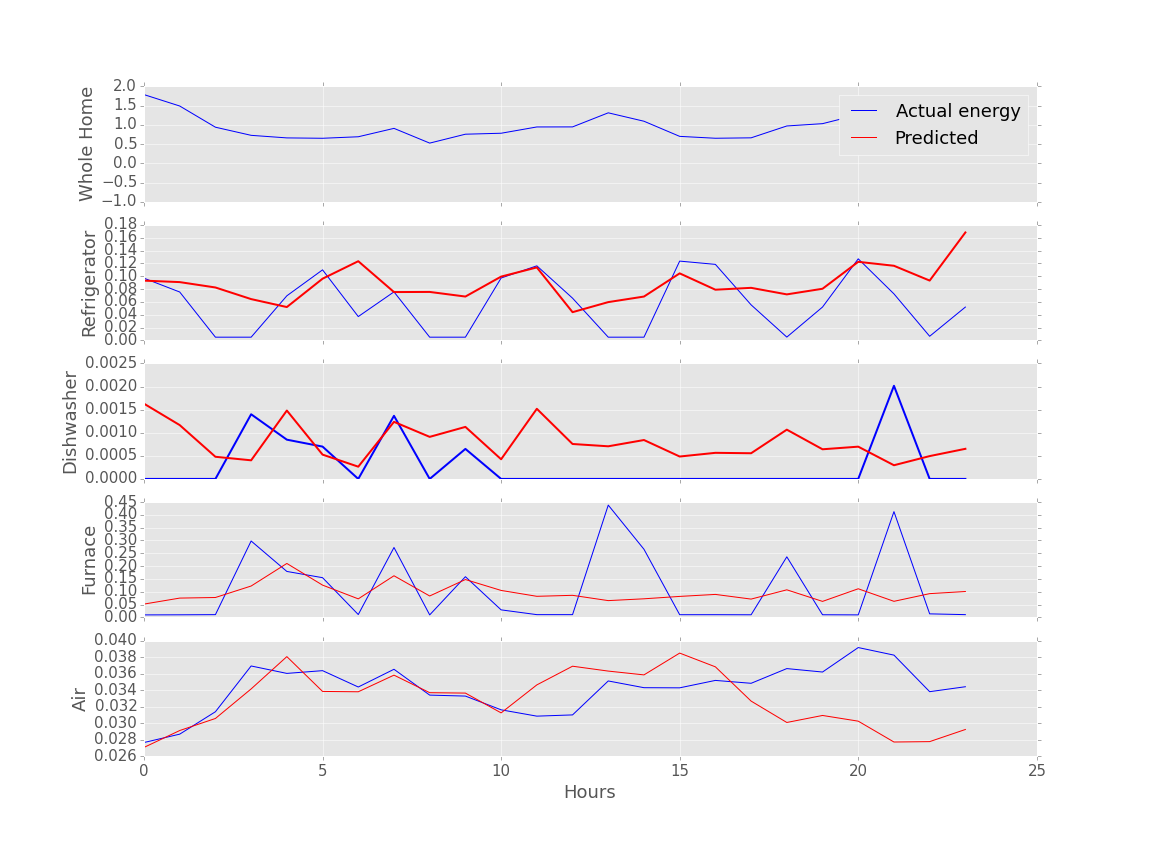
\includegraphics[width=\textwidth,height=8cm]{./figures/normal_250_24}
		%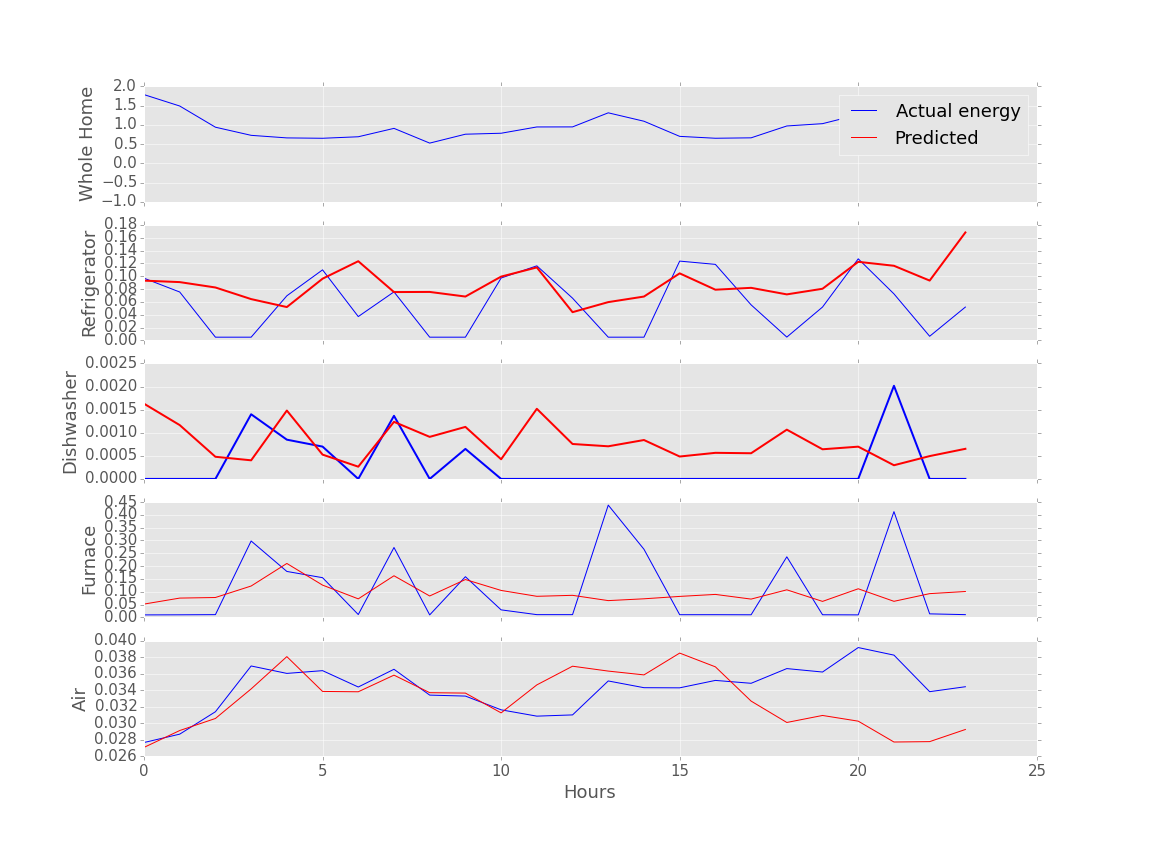
\includegraphics[scale=0.20]{./figures/normal_250_24}
\end{figure}
\begin{figure}[H]
		\centering
		\textbf{Weekdays}\vspace{0.00001in}
		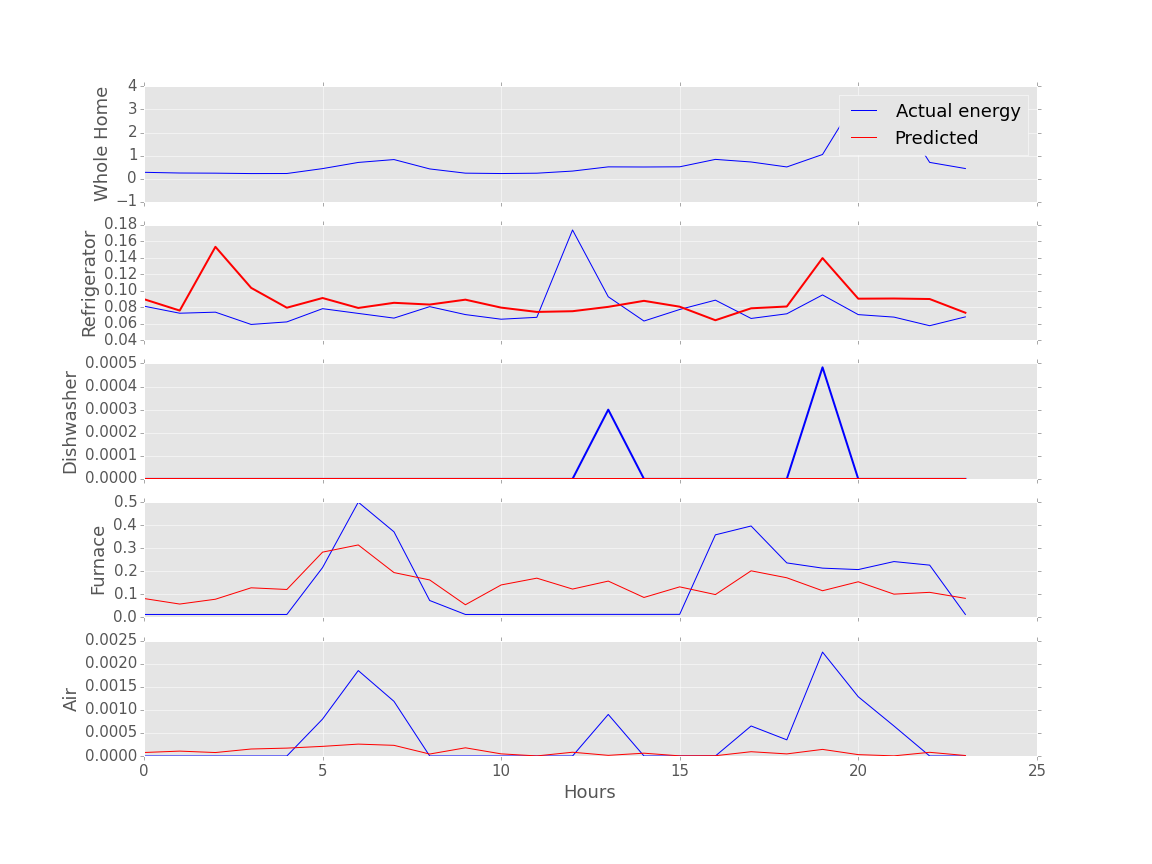
\includegraphics[width=\textwidth,height=8cm]{./figures/days_250_24}
	\end{figure}
\begin{figure}[H]
		\centering
		\textbf{Weekends}\vspace{0.00001in}
		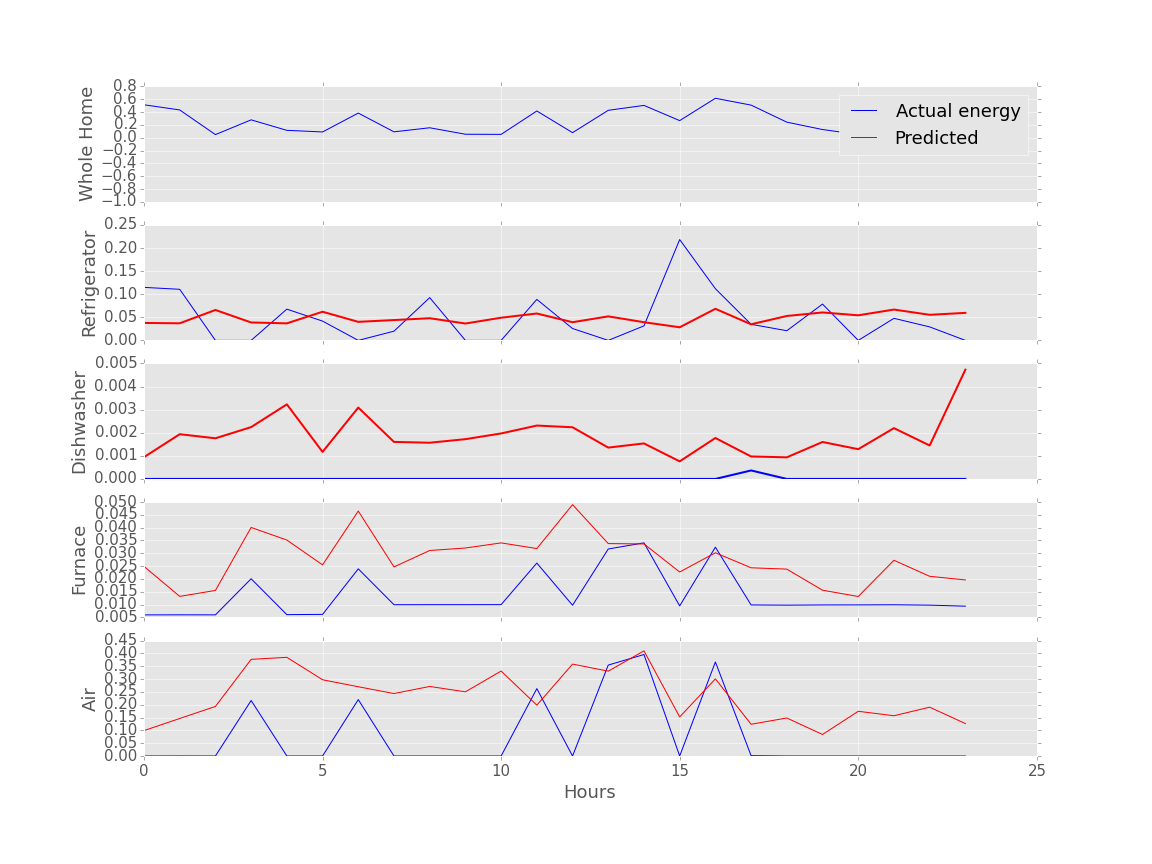
\includegraphics[width=\textwidth,height=8cm]{./figures/end_250_24}
\end{figure}
	
\begin{figure}[H]
	\caption{The figure shows the true usage (blue) and predicted energy consumption (red) of all of the appliances for all datasets. The left hand plot shows the whole dataset used in predicting the 24 hours. The middle plot shows the weekdays dataset being predicted for 24 hours and the right hand plot shows the prediction for the weekend dataset.}
	\label{fig:subset}
\end{figure}


In all the cases the algorithm has found basis functions and activations to represent an energy consumption profile of all of the appliances. This goes to show that the implementation of the algorithm has been successful and that the algorithms do serve their purpose, more on the evaluation on the different algorithms is done further down in section \ref{sec:quant}. Interesting to note is that the algorithm has found some of the energy profiles of some appliances. Looking at the plot to the bottom left we see that the prediction has actually been proved to be almost in line with the true profile for 10 of the data points (10 hours). We can also see that the algorithm can output completely different profiles by looking at the refrigerator for the weekdays dataset compared to that of the air-condition profile for the week dataset. 

\subsubsection{Results from the complete dataset}
\label{sec:complete}
\begin{figure}[H]
	\centering
	\textbf{$T=$168 hours and $m=$67 houses and $n=$80 basis functions}\par\medskip
	\begin{minipage}{.65\textwidth}
		\centering
		%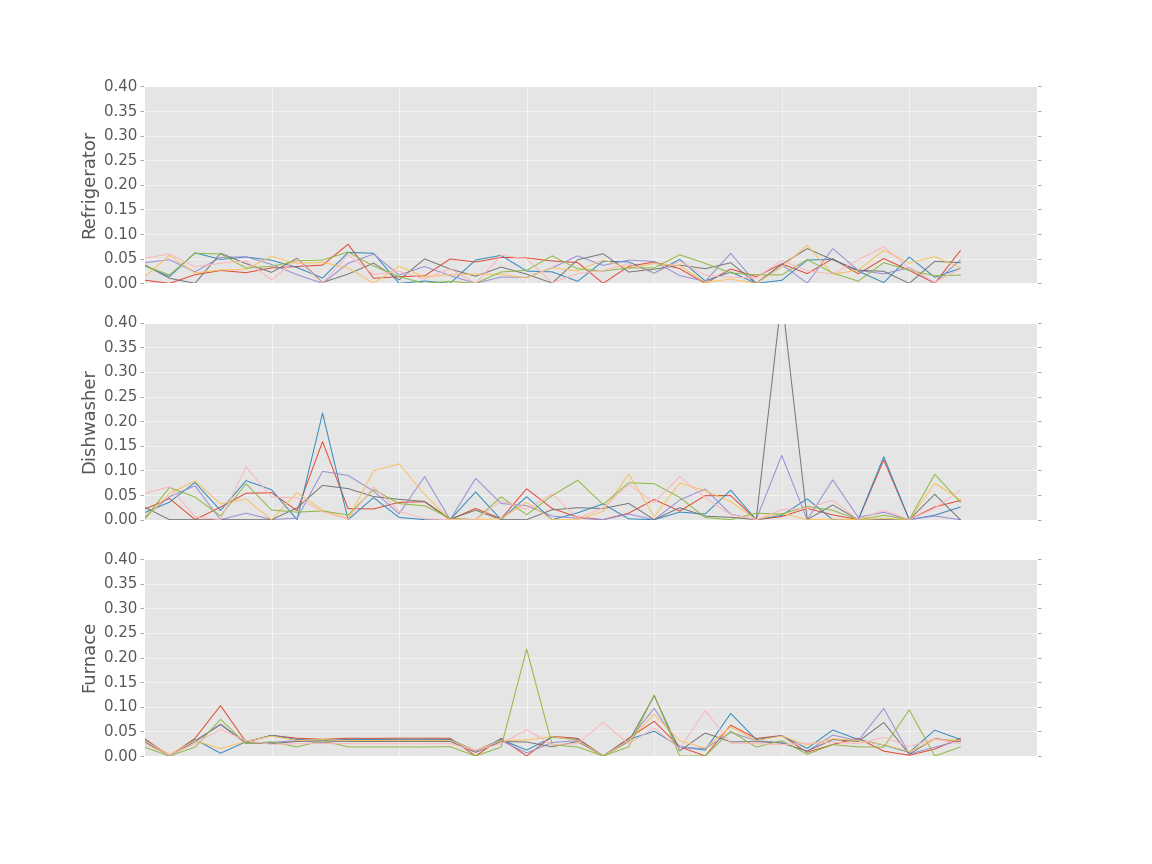
\includegraphics[scale=0.18]{./figures/app_basis}
		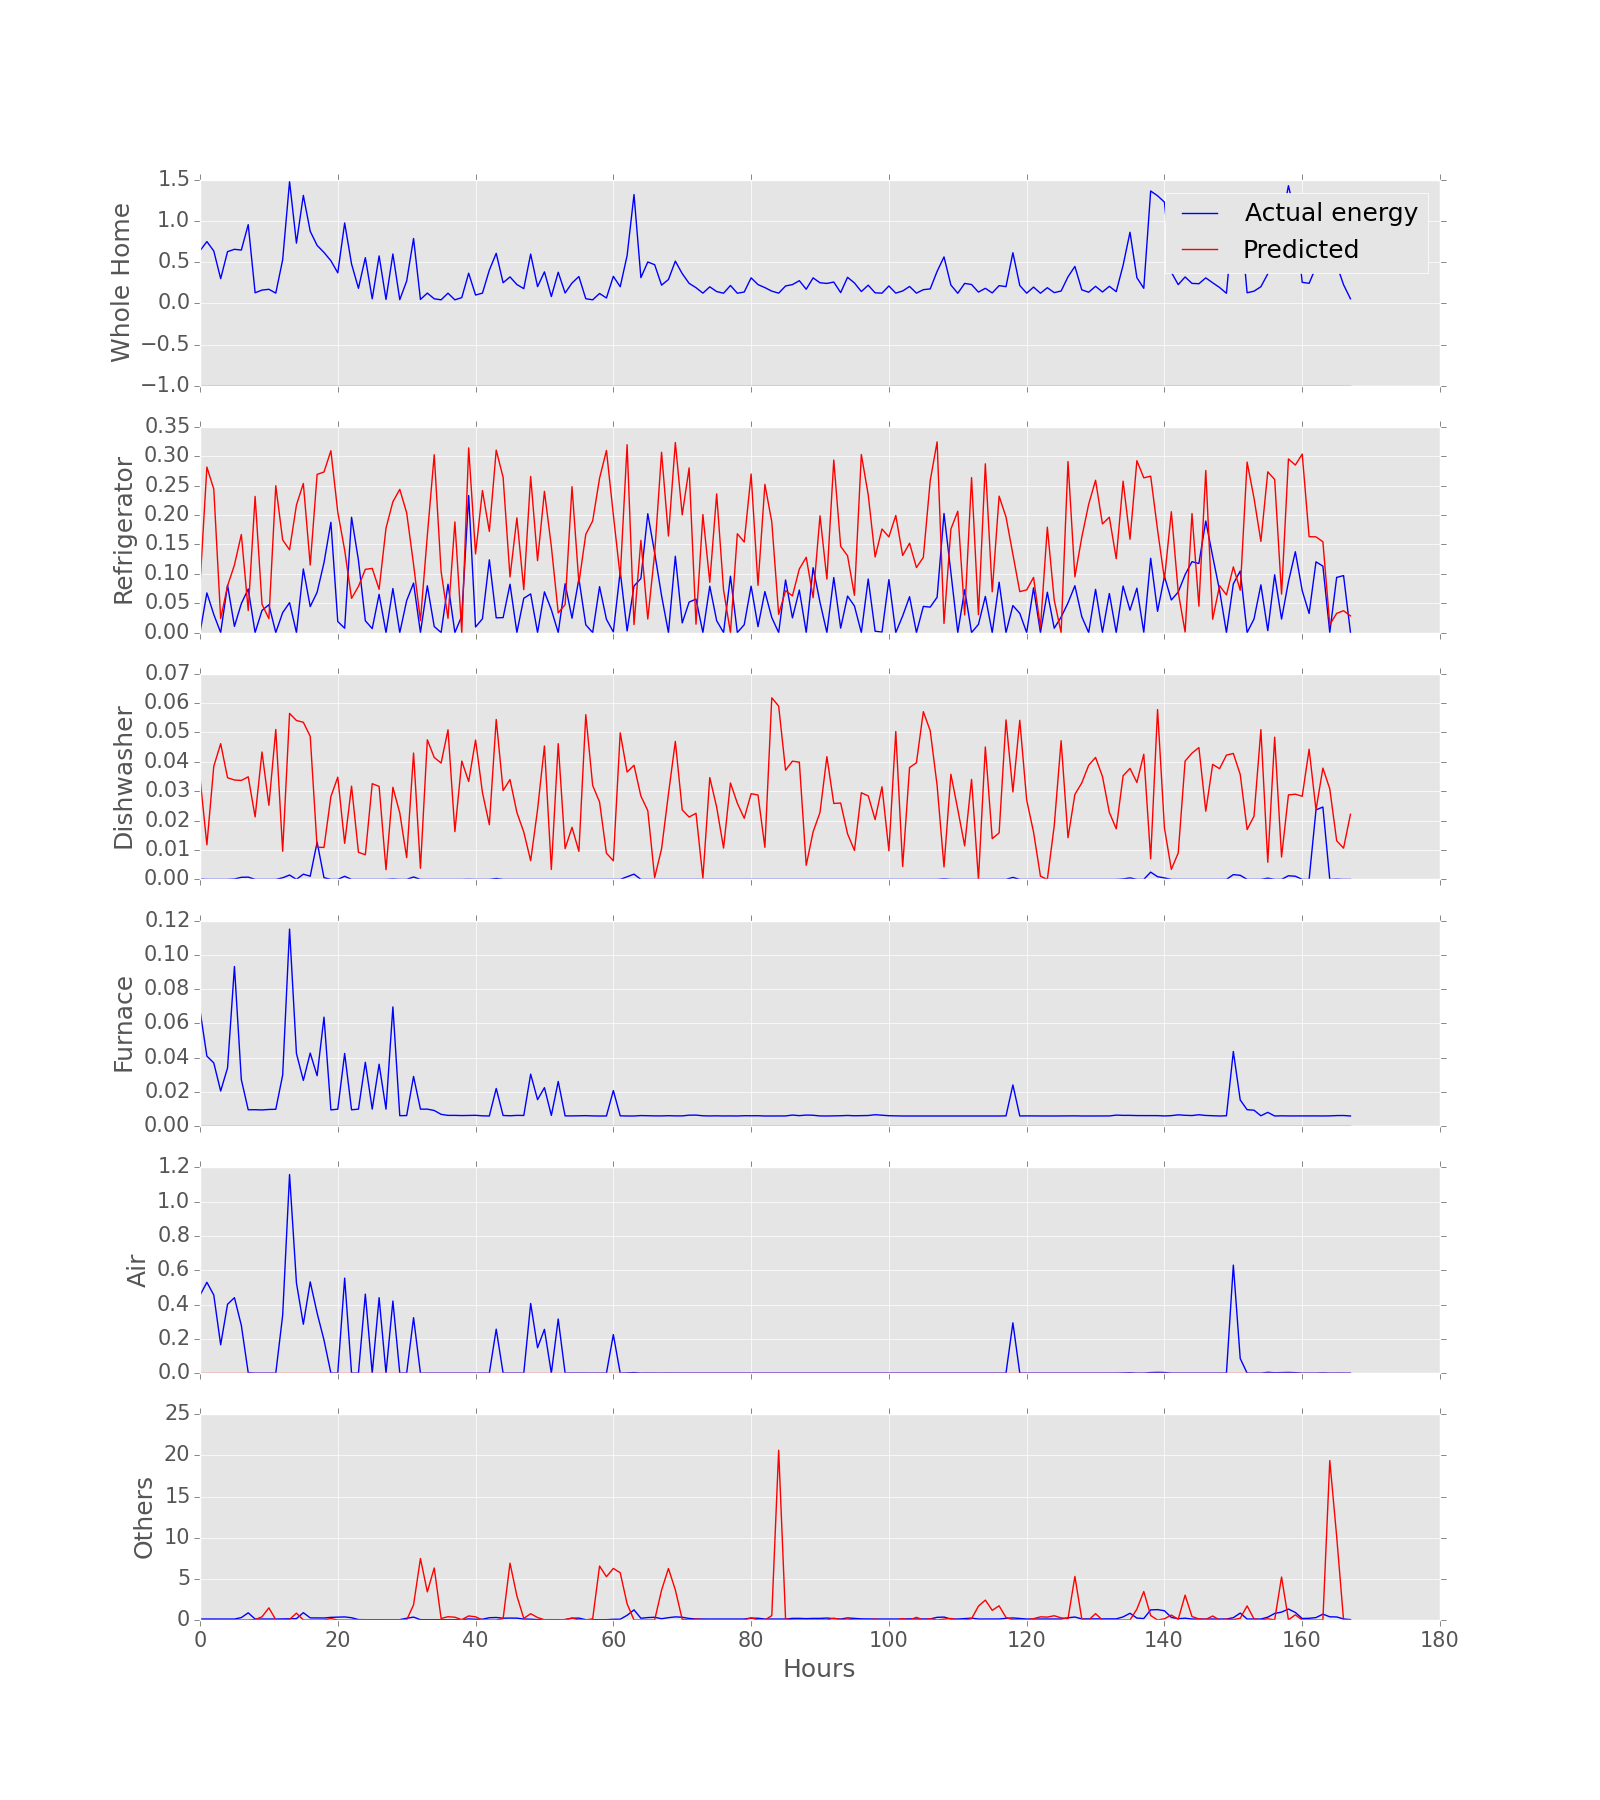
\includegraphics[width=\textwidth,height=10cm]{./figures/results/normal_appliances_67_168}
	%	\label{fig:test8}
	\end{minipage}%
	\begin{minipage}{.4 \textwidth}
		\centering
		%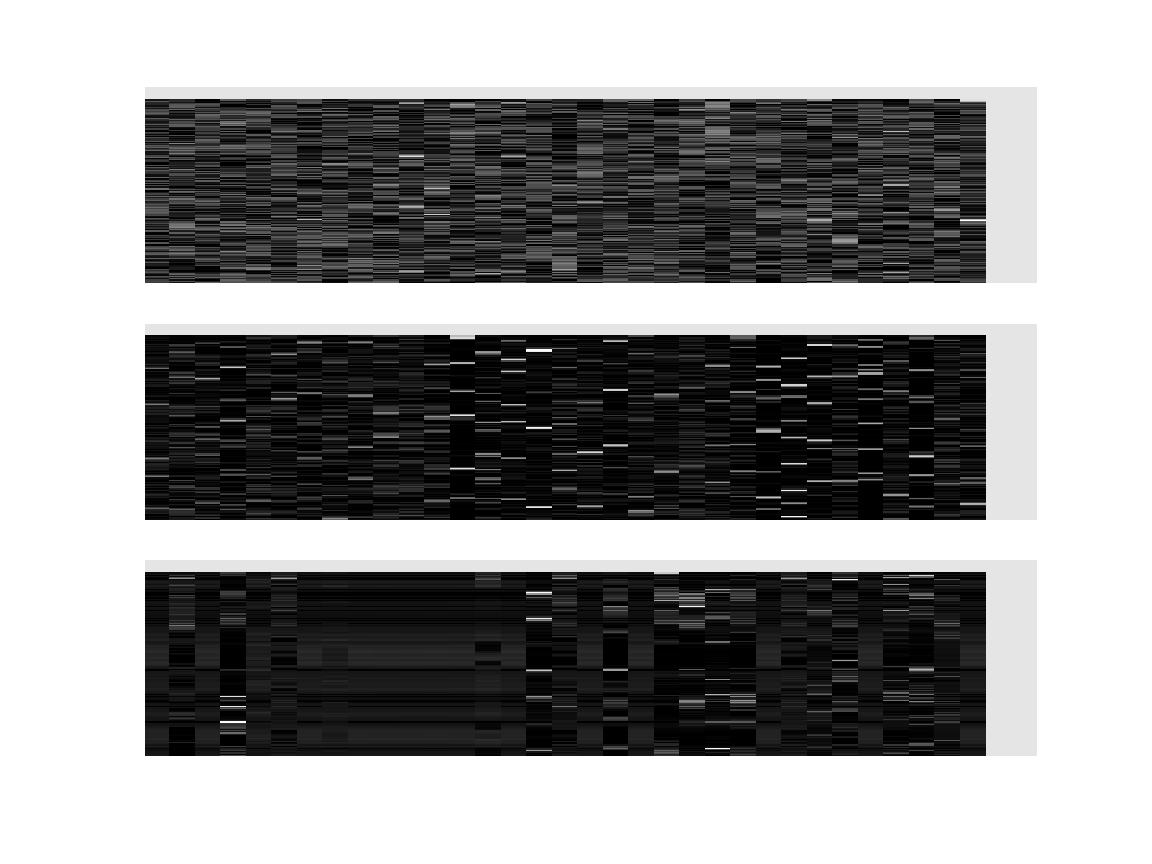
\includegraphics[scale=0.18]{./figures/basis}
		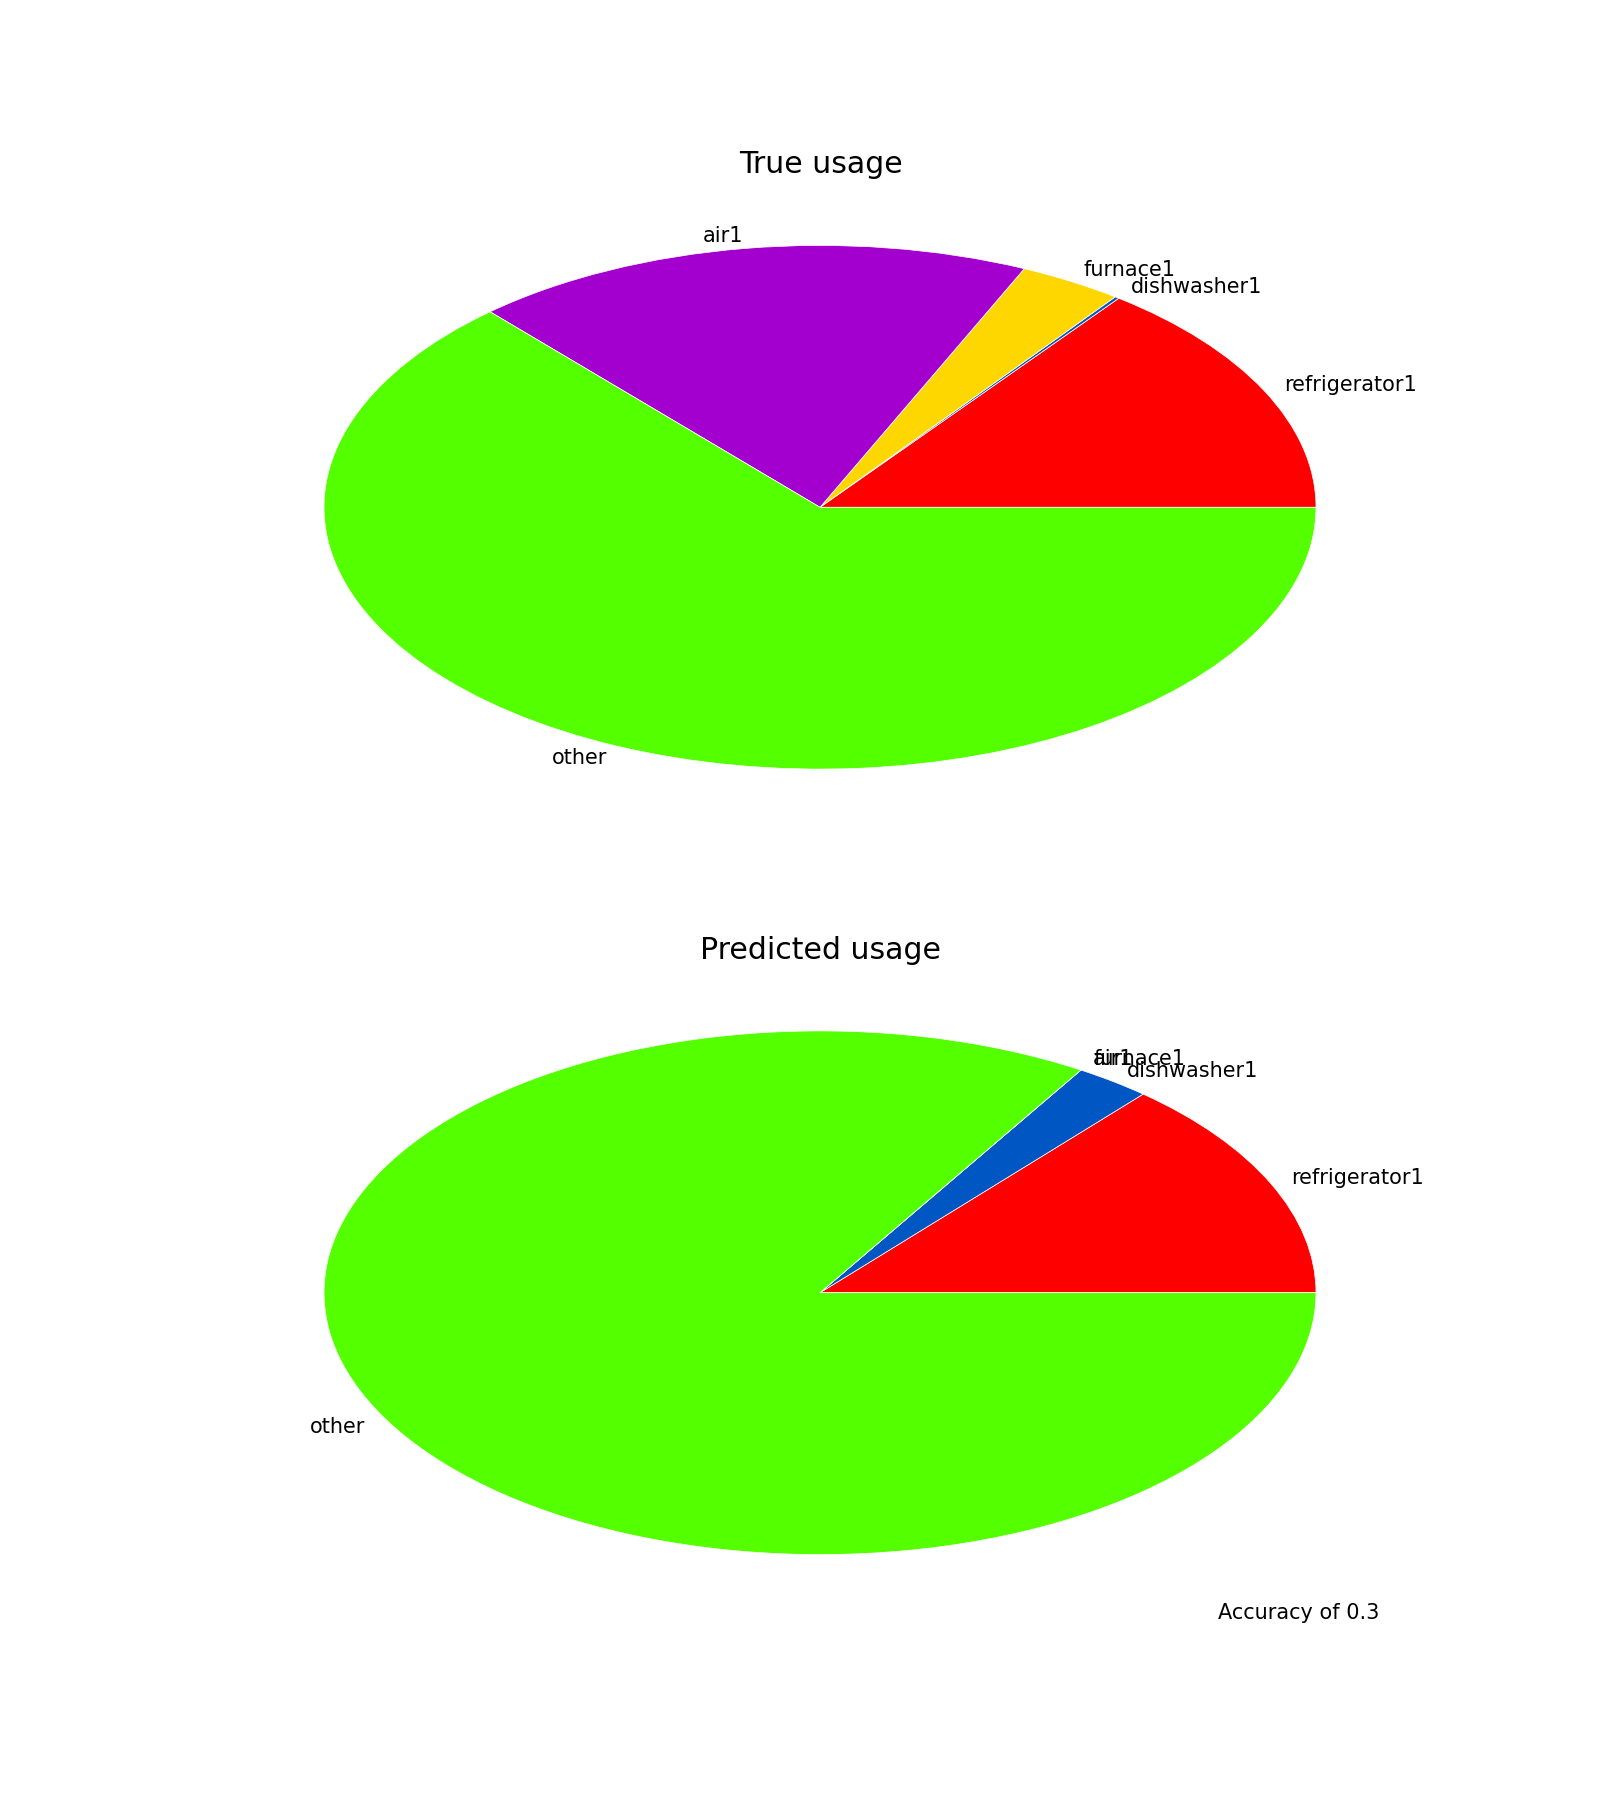
\includegraphics[width=\textwidth,height=10cm]{./figures/results/normal_pie_chart_67_168}
	%	\label{fig:test9}
	\end{minipage}
	\caption{Example of one house true energy profile and the predicted energy profile over a one week time period. The plot to the left shows true and predicted energy profiles. The plot to the right shows a pie chart of the total percentage that each appliance true usage and predicted usage.}
	\label{fig:normal_168}
\end{figure}

In most cases, the predicted values are quite poor, and the overall accuracy was 0.29, by the definition in equation \ref{eq:acc}. It seems as though the algorithm has not gotten any type of pattern but rather unique constant energy consumption for each appliance. Both the dishwasher and the refrigerator have a consistent shape of being volatile and almost like noise. One thing to note is the shape of the predicted usage of other appliances, this shape is highly complex due to its peak like behavior and is one shape that is hard to try to learn without using methods such as sparse coding which says that the algorithm can be used for predicting the shapes. Although it has overestimated the usage of other appliances as we can see in the pie charts. However it has completely not learnt that air or furnace has not been used at all, which is a failure in the results, and only the refrigerator has roughly the same amount of percentage usage as the true usage. The "other" appliances can be seen as a good result when representing a complex structure such as a dishwasher usage we have captured the structure of a "on" and "off" behavior, even though we did not use enough basis functions, we can still represent a structure like it. It is however not a good result when predicting each appliance as well as the overall energy usage. It heavily overestimates the usage of "other" appliances as well as assumes a significant higher consumption on both the "other" appliances and the dishwasher. 

\begin{figure}[H]
	\centering
	\textbf{$T=$360 hours and $m=$67 houses and $n=$144 basis functions}\par\medskip
	\begin{minipage}{.65\textwidth}
		\centering
		%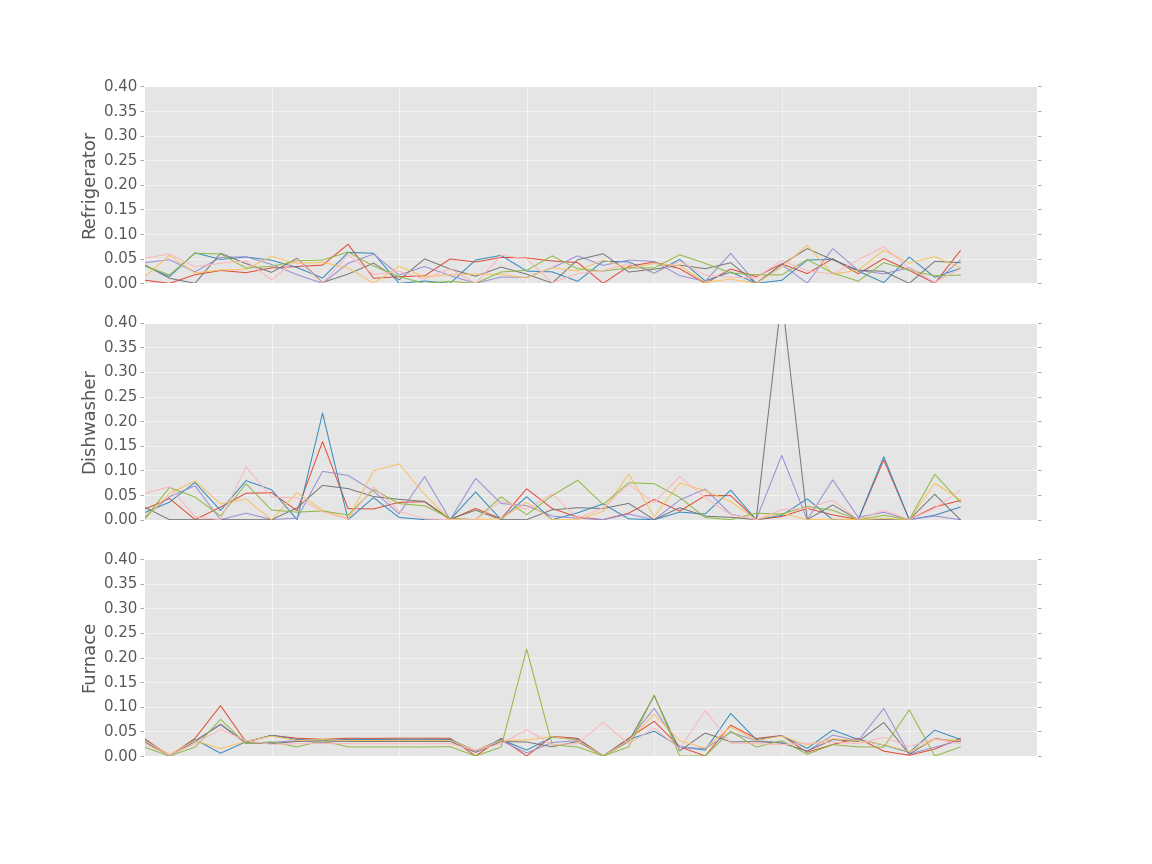
\includegraphics[scale=0.18]{./figures/app_basis}
		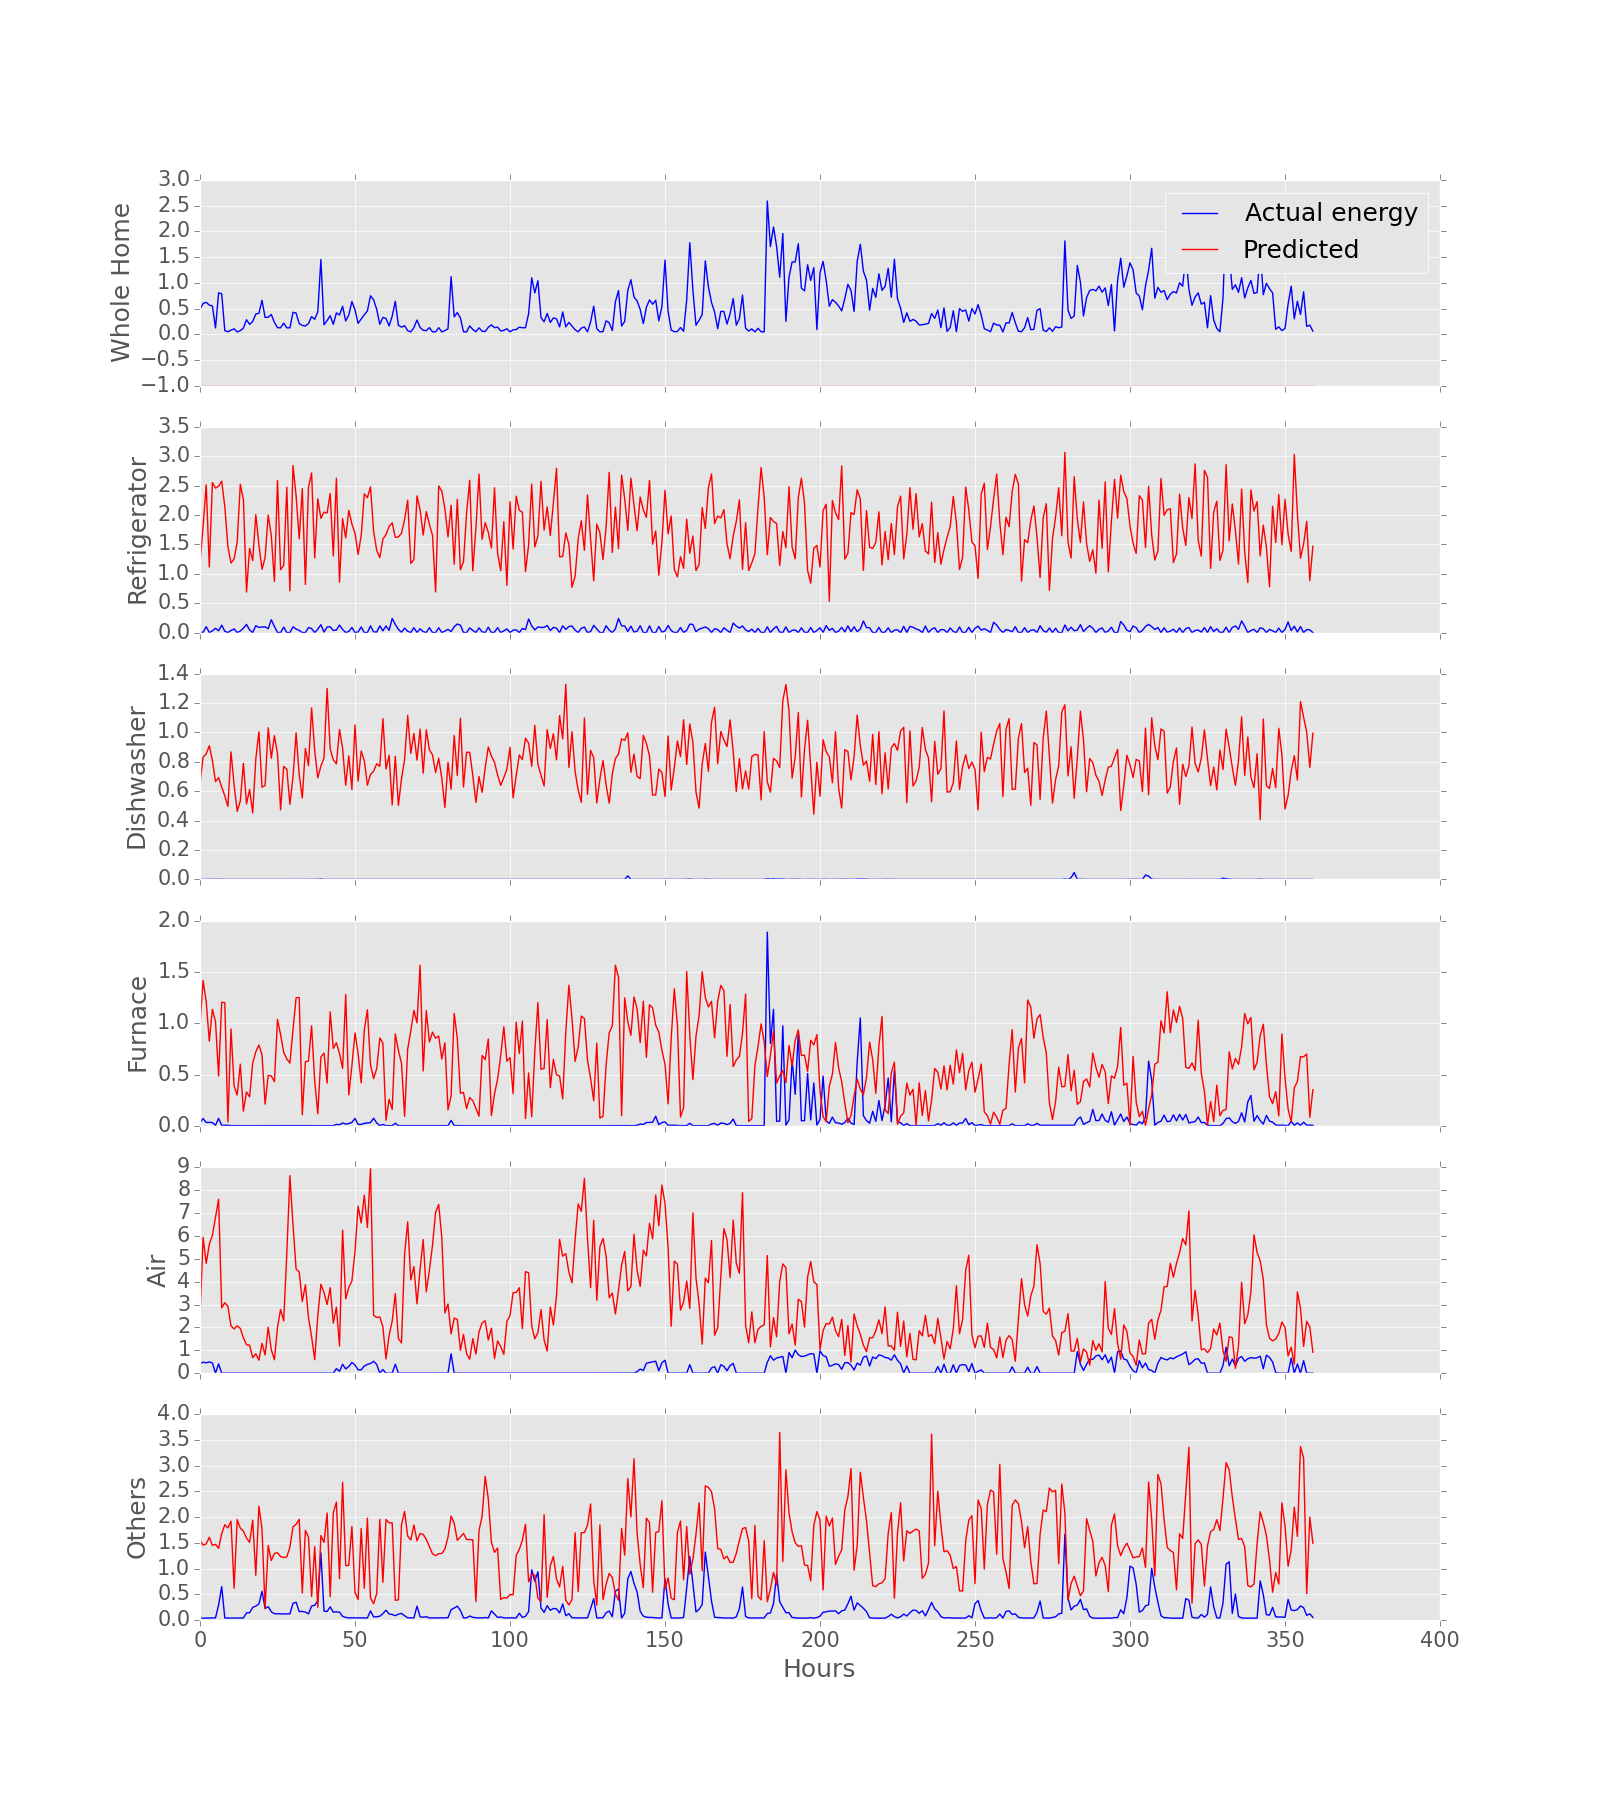
\includegraphics[width=\textwidth,height=10cm]{./figures/results/normal_appliances_144_360}
		\label{fig:test8}
	\end{minipage}%
	\begin{minipage}{.4\textwidth}
		\centering
		%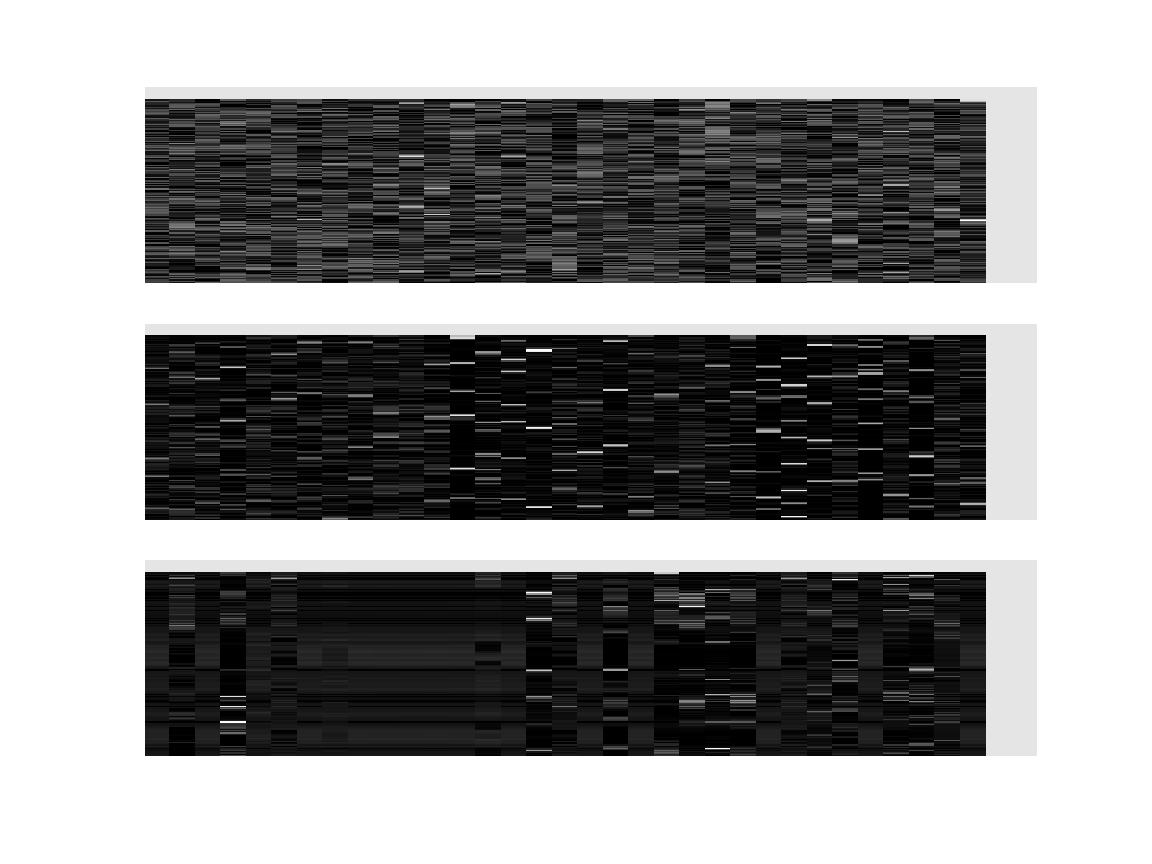
\includegraphics[scale=0.18]{./figures/basis}
		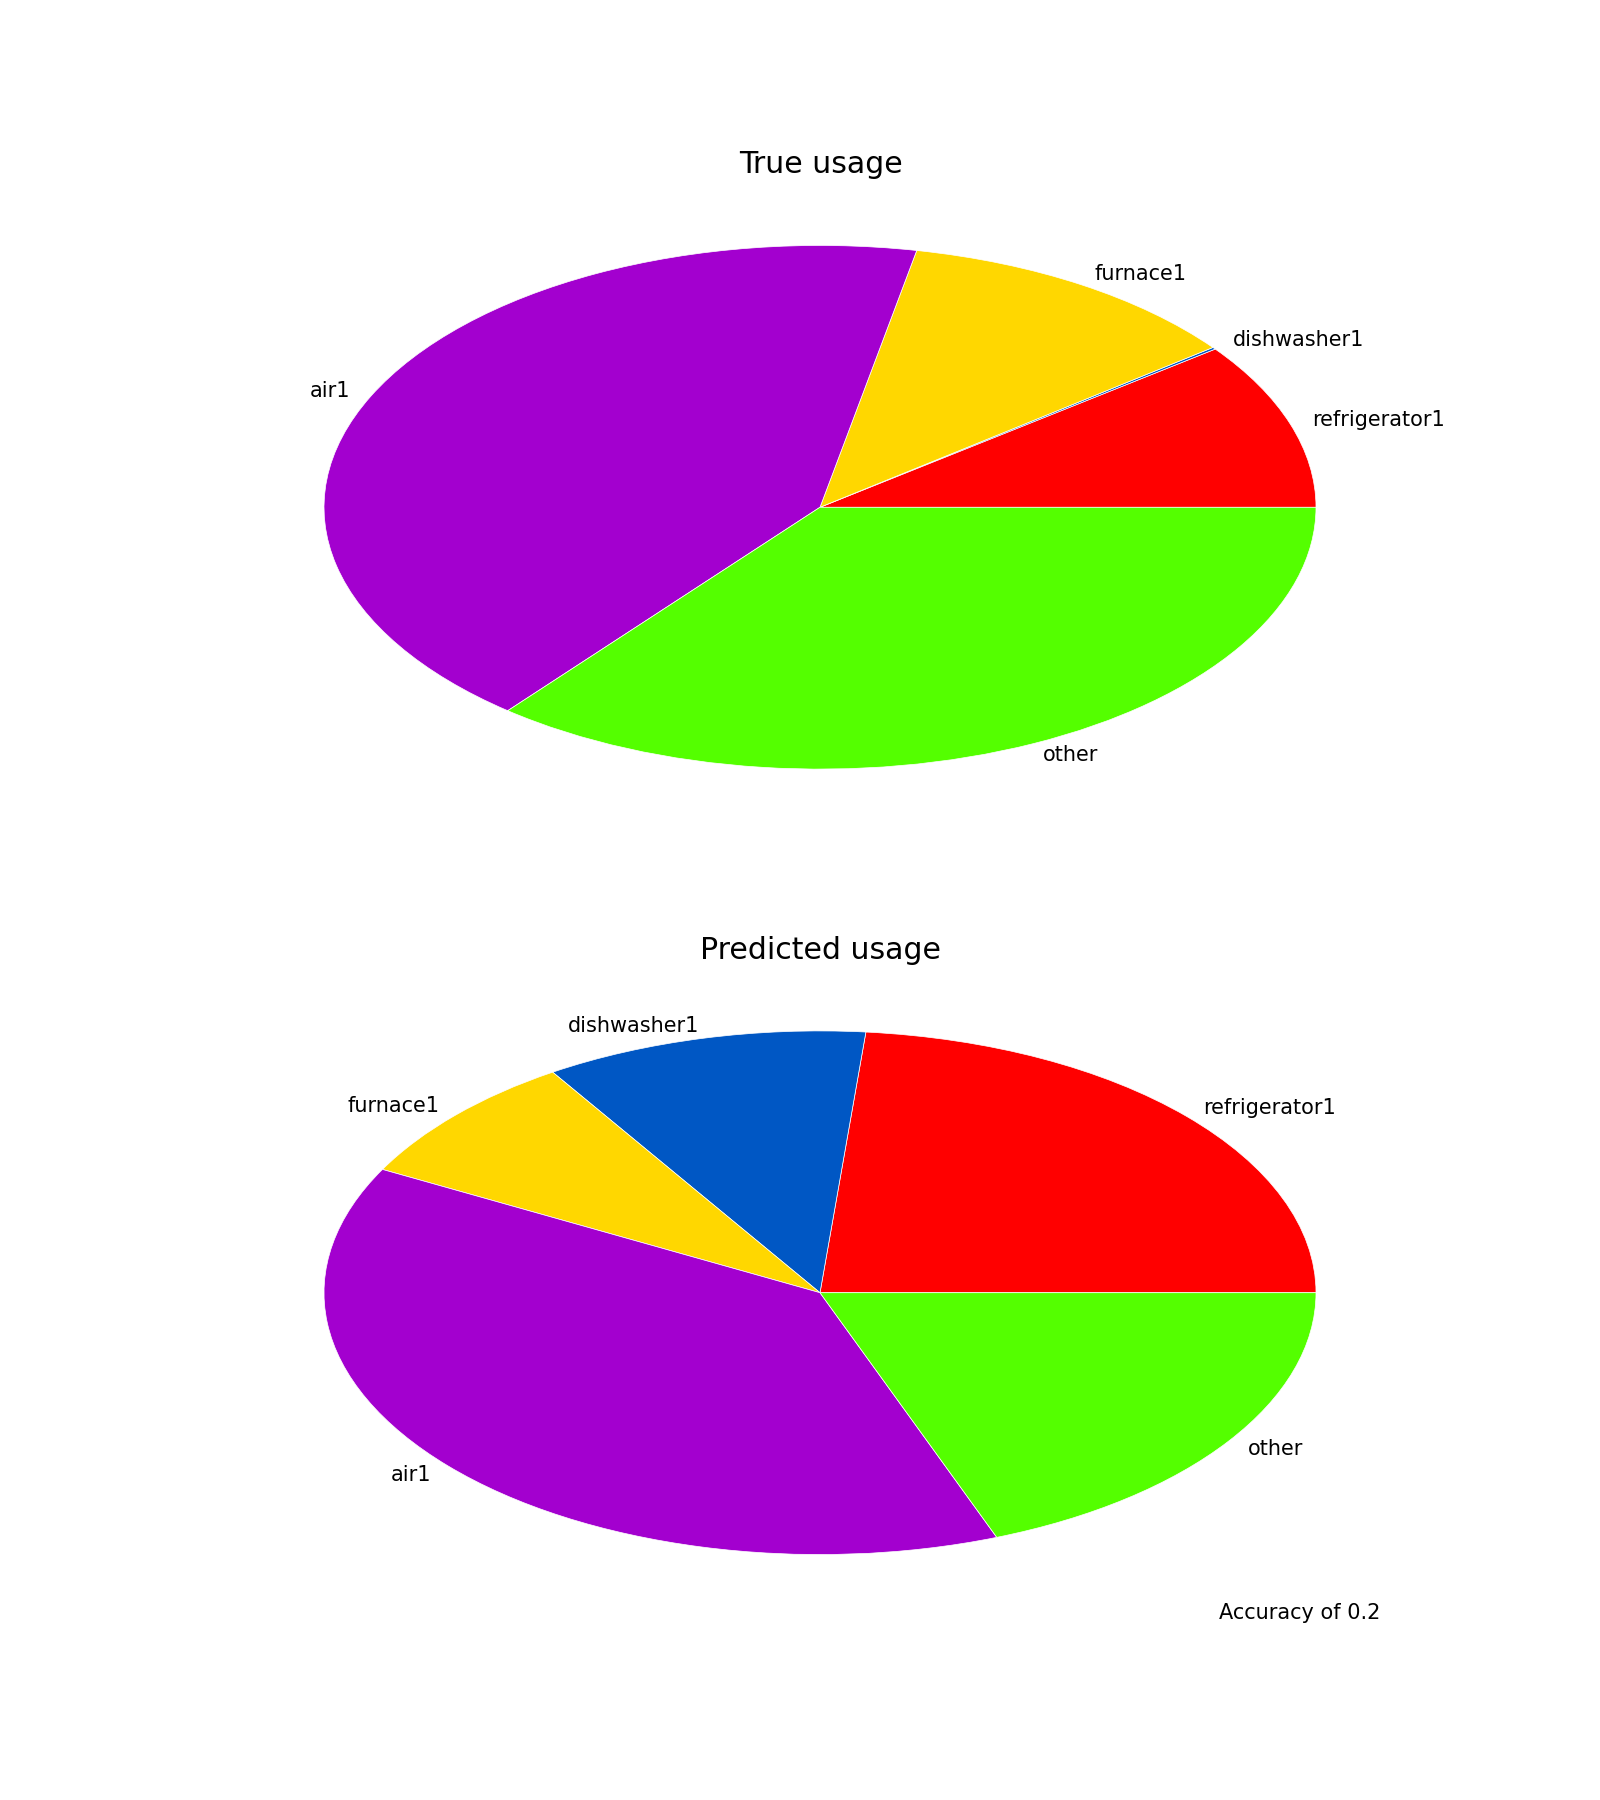
\includegraphics[width=\textwidth,height=10cm]{./figures/results/normal_pie_chart_144_360}
	\end{minipage}
	\caption{Example of one house true energy profile and the predicted energy profile over a two week time period. The plot to the left shows true and predicted energy profiles. The plot to the right shows a piechart of the total percentage that each appliance true usage and predicted usage.}
	\label{fig:normal_360}
\end{figure}

When the algorithm was tested on a two week set of hourly readings, the results were again poor and had a overall accuracy rate of 0.21. The house shows in the plot to the left of the figure \ref{fig:normal_360} has minimal consumption of the dishwasher and refrigerator, but it is visually hard to see as the predicted values are of a magnitude higher. The predicted shapes of the dishwasher and the refrigerator look more or less as a Brownian motion, same as for the prediction of one-week of data but here the predicted values are significantly higher. This behavior could come from the DDSC algorithm where we discriminate the whole signal, and the norm of the activations during this algorithm spikes significantly high, up to 25 000 from a mere 2211, as shown in figure \ref{fig:a_b_ddsc}. This could be that the algorithm overestimates the whole home usage and therefore predicts a higher consumption of the appliances. Furthermore, is that the basis functions are trained to represent the activations trained during this algorithm and that these overestimate some appliances like the dishwasher and the refrigerator seem to have, in both the case for the weekly predictions and of the two week predictions. We can see that all of the appliances are overestimated in their power consumption usage. However, when comparing the predictions for the two tests (week and two weeks) we see that in the later case we see that most of the appliances have been overestimated but in the first case we see that the "other" appliances have been heavily overestimated while both the air and the furnace have been predicted to not be in use at all. This could say that the algorithm can make a better prediction for more appliances when used on a larger dataset. When looking at the pie chart, representing the total percentage use of the predicted versus the true usage, we see from both of the tests, the refrigerator has had the best predicted values. This is probably due to the nature of a refrigerator having a consistent shape, rather than most energy consuming appliance, that have an "on" and "off" behavior.

%% weekdays

\newpage
\subsubsection{Results from weekdays and weekend hourly readings}
\label{sec:days_end}
\begin{figure}[H]
	\centering
	\textbf{168 hours and 67 basis functions \quad 360 hours and 144 basis functions}\par\medskip
	\textbf{Weekday dataset}
	\begin{minipage}{.45\textwidth}
		\centering
		%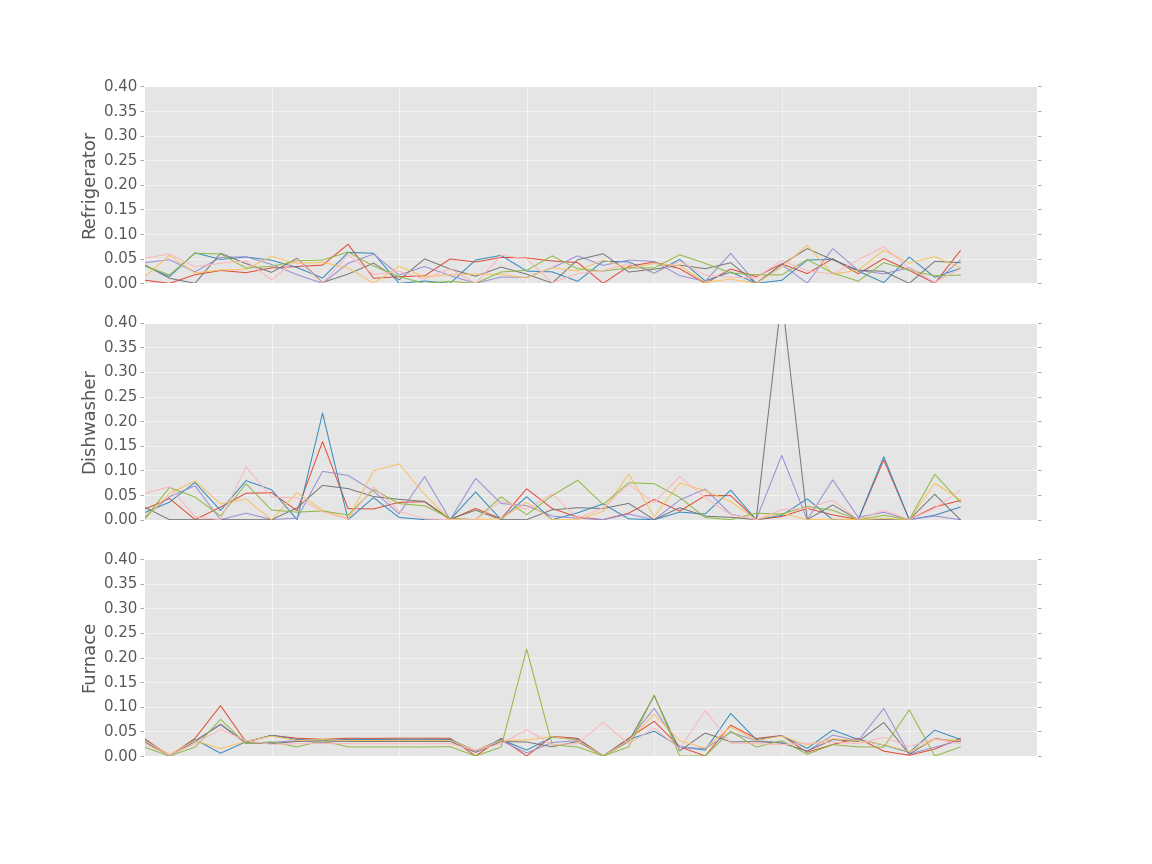
\includegraphics[scale=0.18]{./figures/app_basis}
		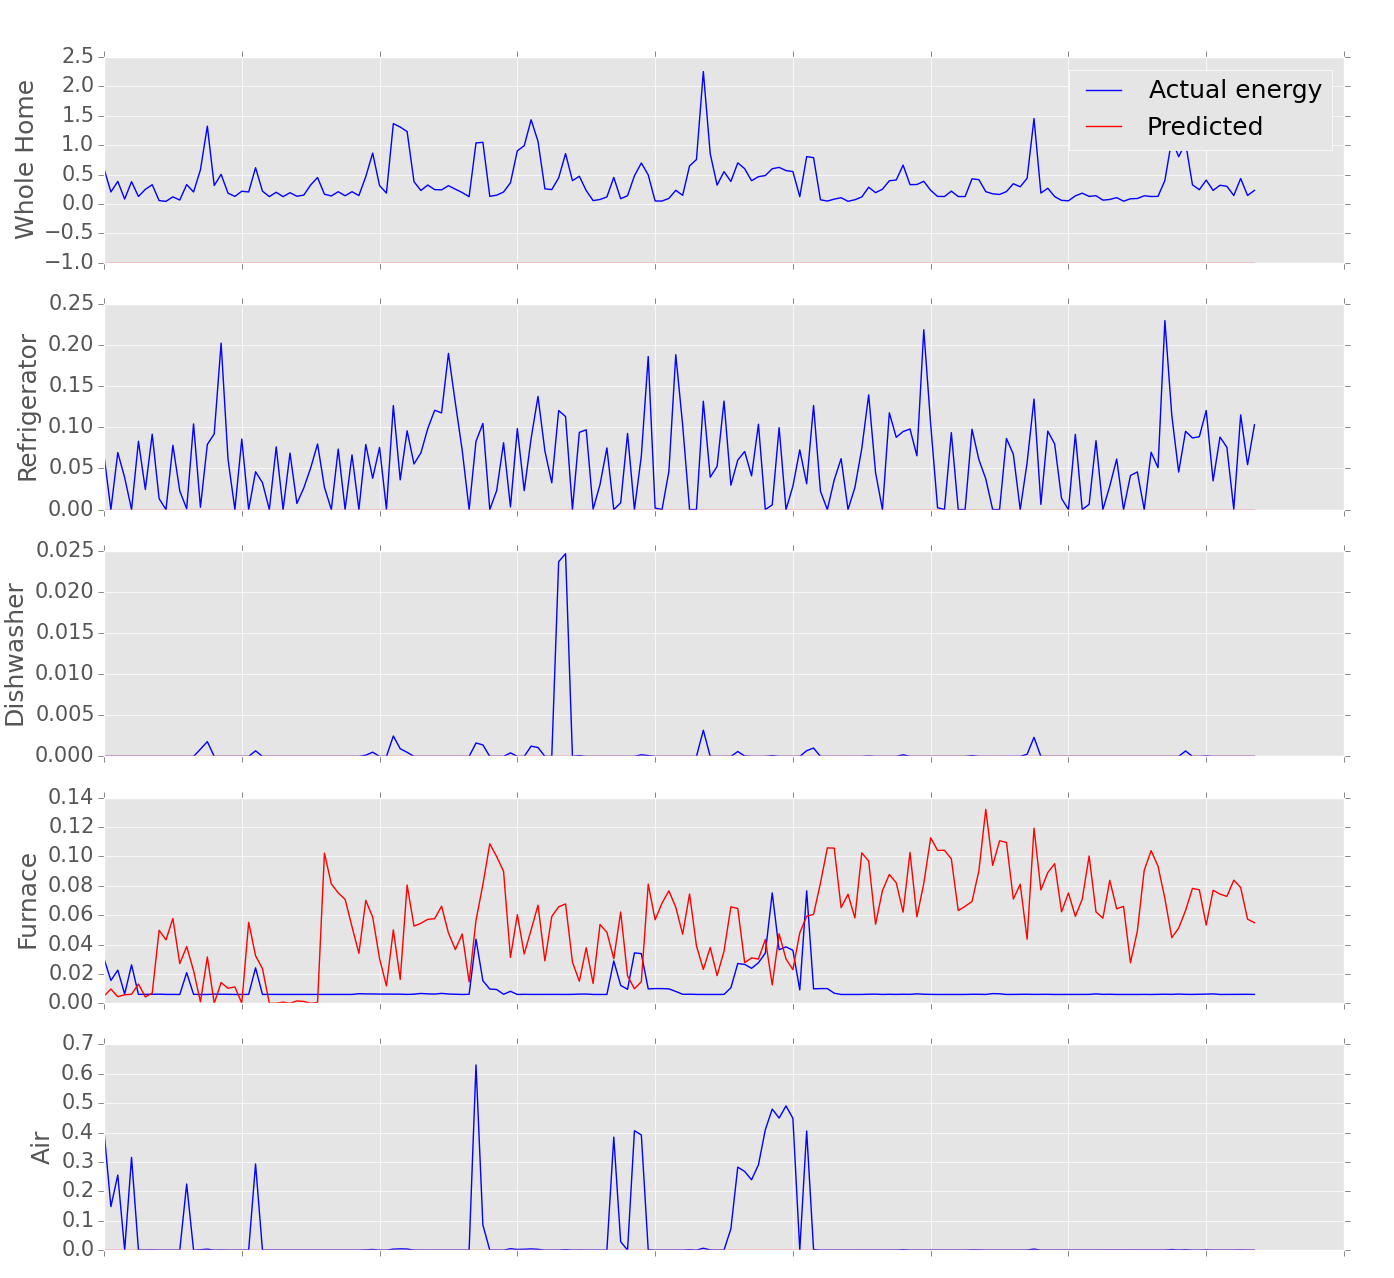
\includegraphics[scale=0.18]{./figures/results/days_appliances_67_168}
	\end{minipage}%
	\begin{minipage}{.45\textwidth}
		\centering
		%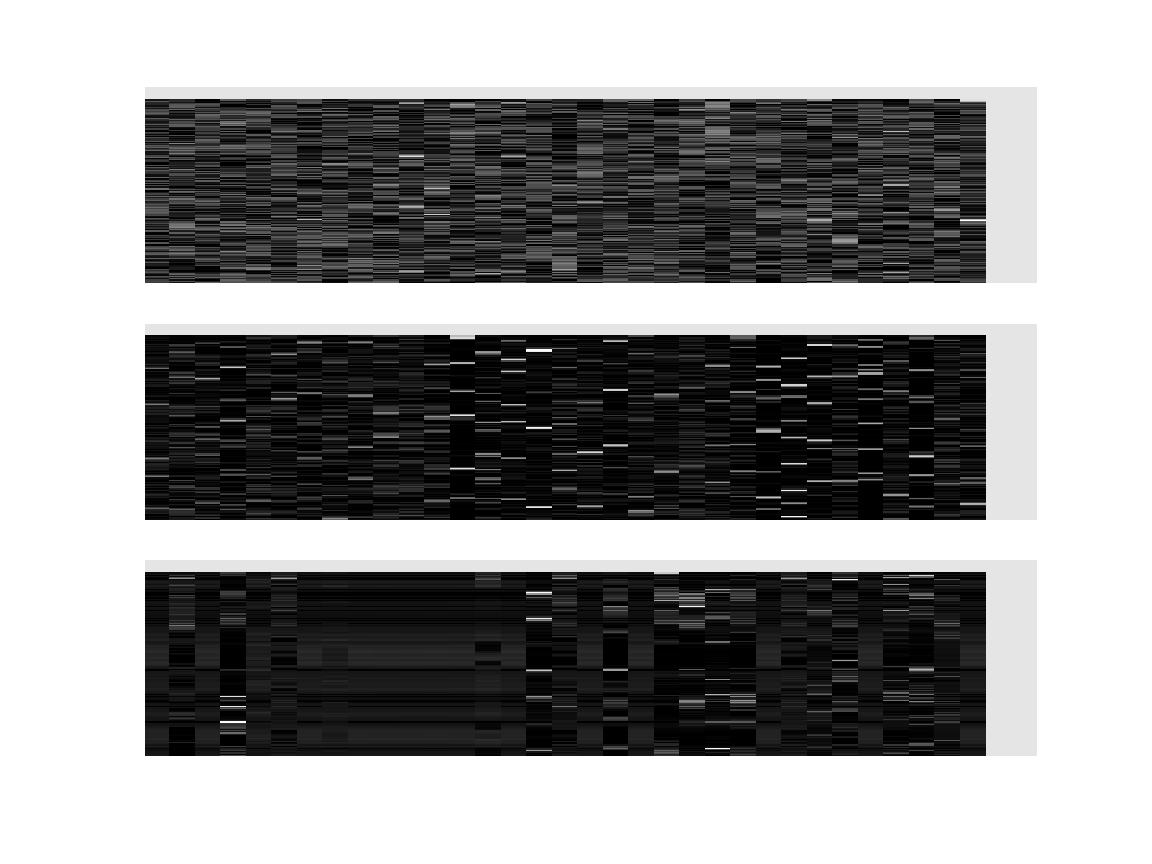
\includegraphics[scale=0.18]{./figures/basis}
		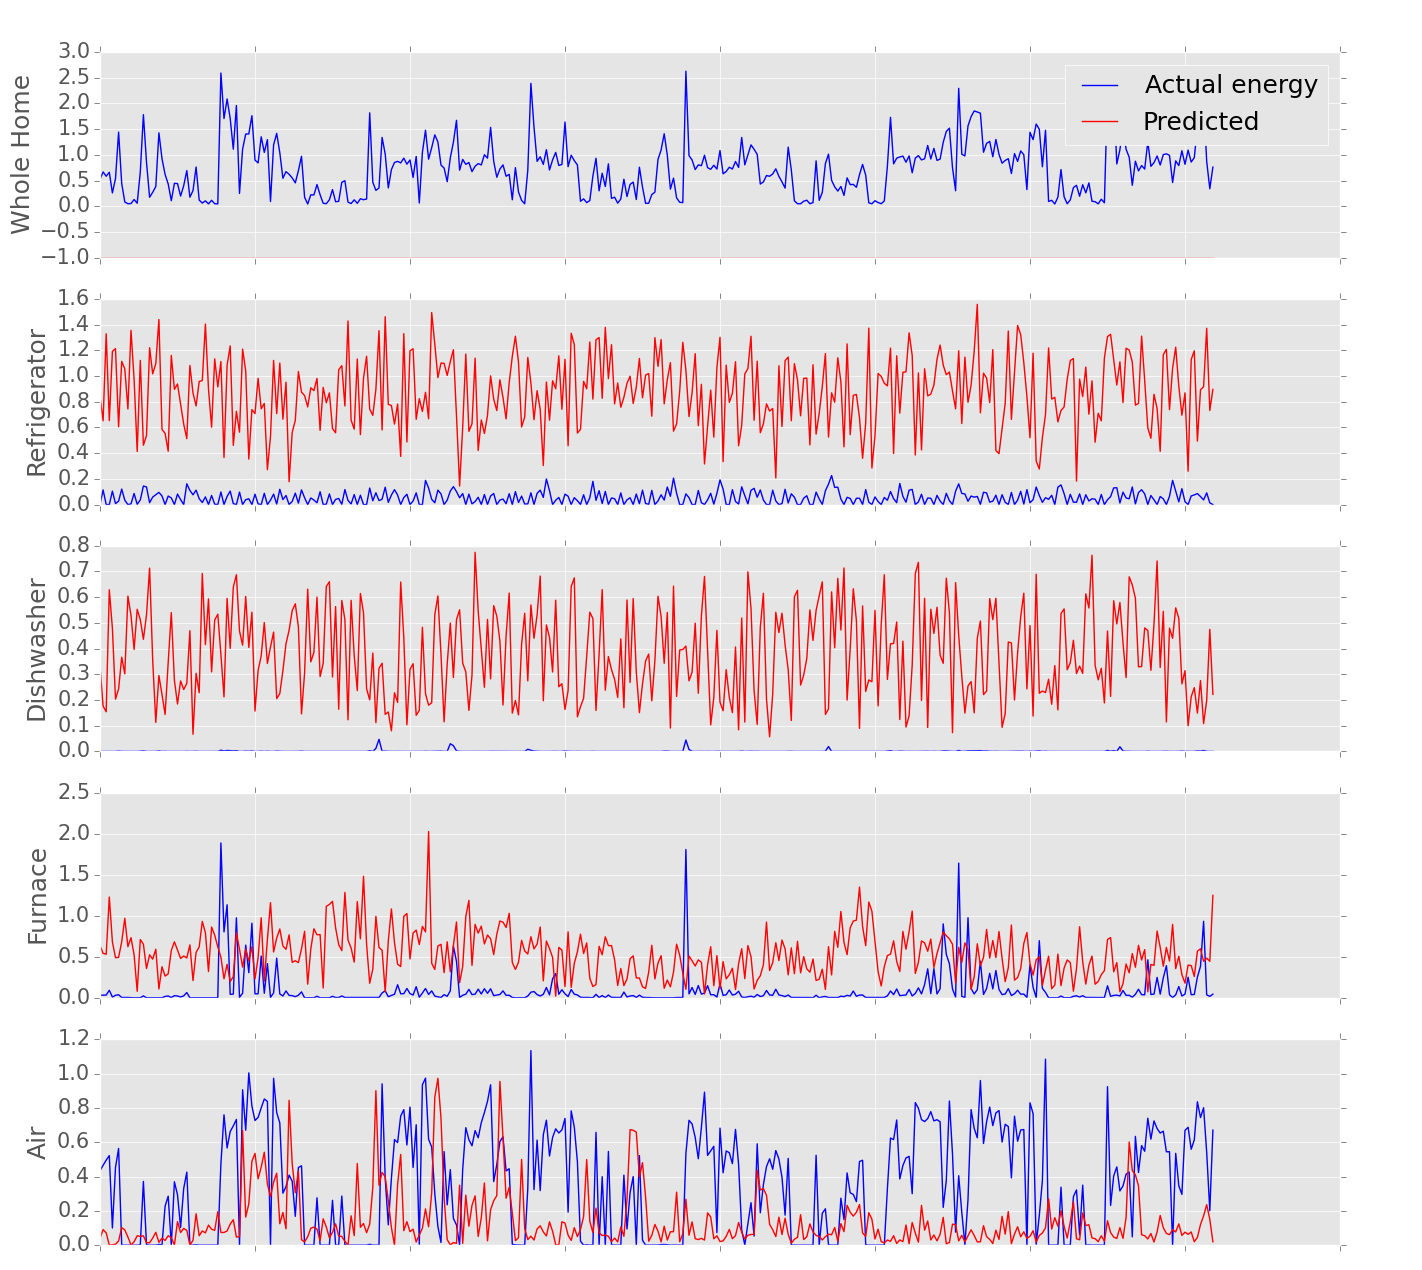
\includegraphics[scale=.18]{./figures/results/days_appliances_144_360}
	\end{minipage}
\end{figure}
%%% weekends
\begin{figure}[H]
	\centering
	\textbf{Weekend dataset}
	\begin{minipage}{.45\textwidth}
		\centering
		%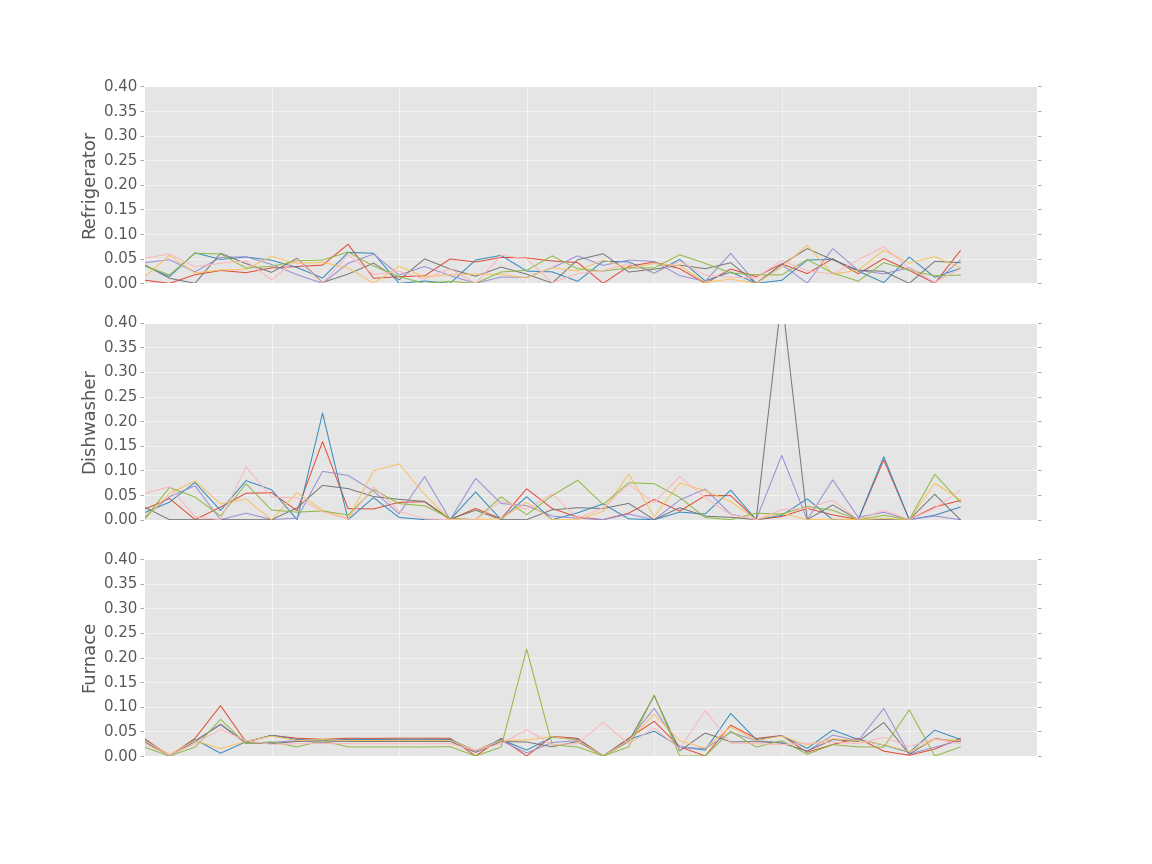
\includegraphics[scale=0.18]{./figures/app_basis}
		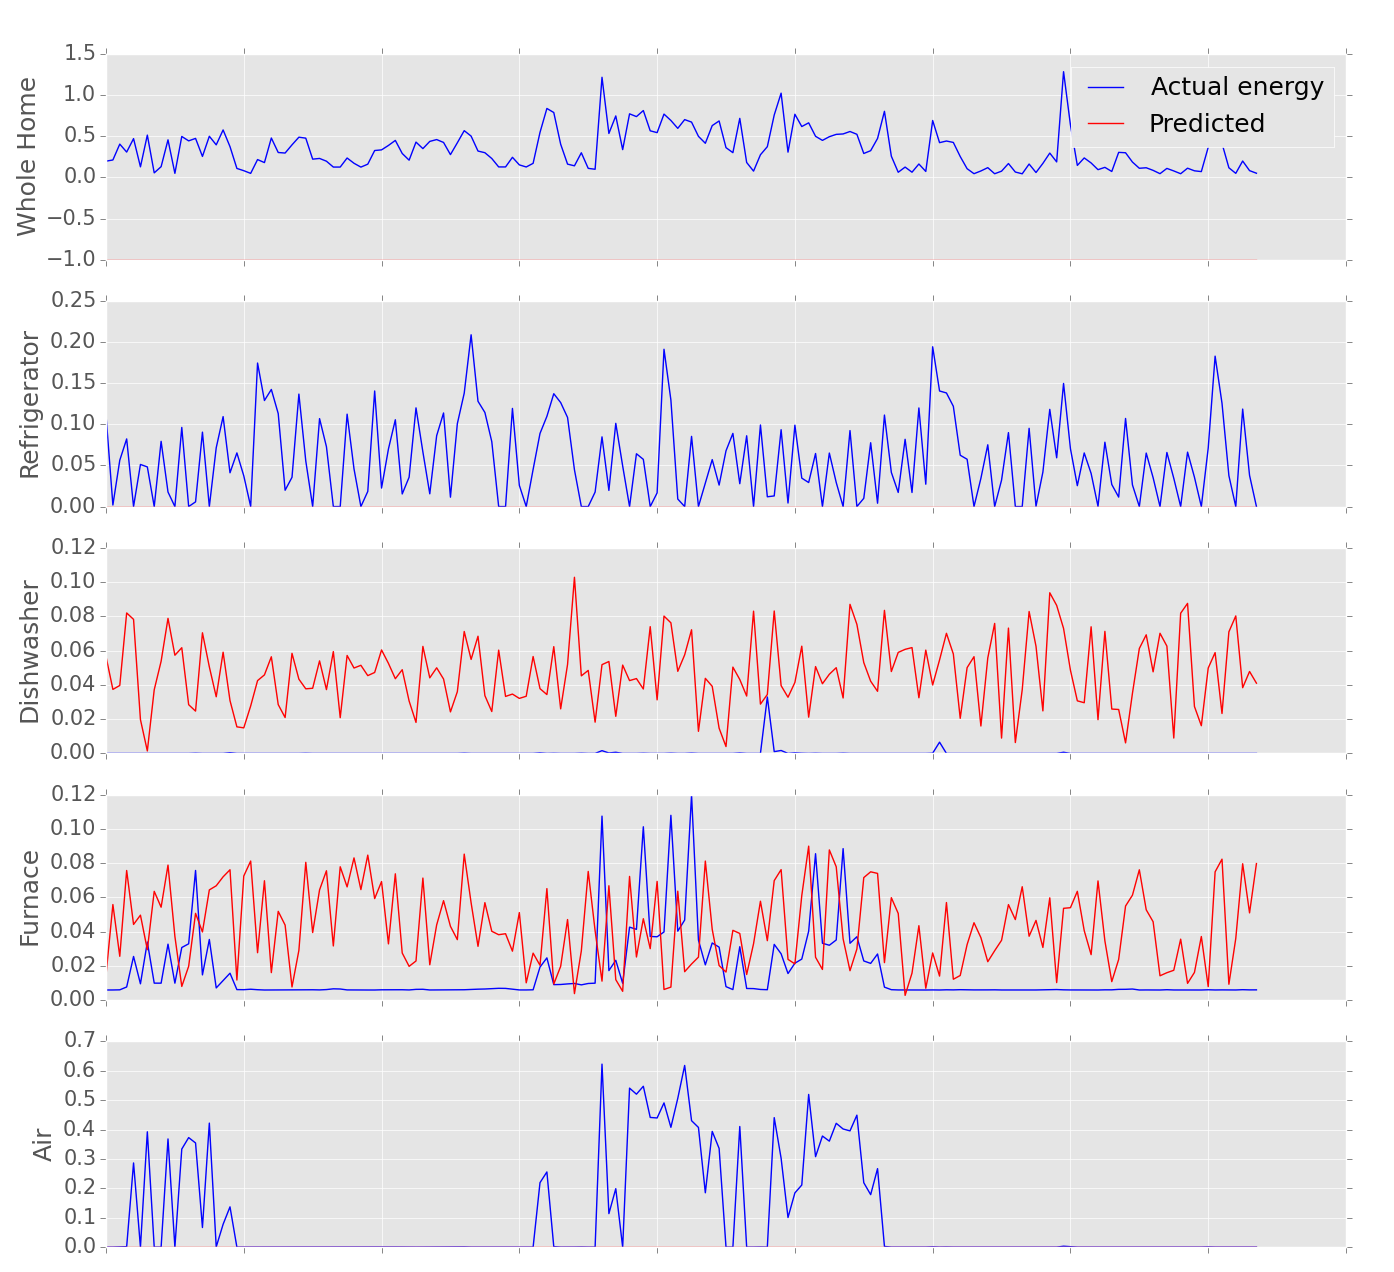
\includegraphics[scale=0.18]{./figures/results/end_appliances_67_168}
	\end{minipage}%
	\begin{minipage}{.45\textwidth}
		\centering
		%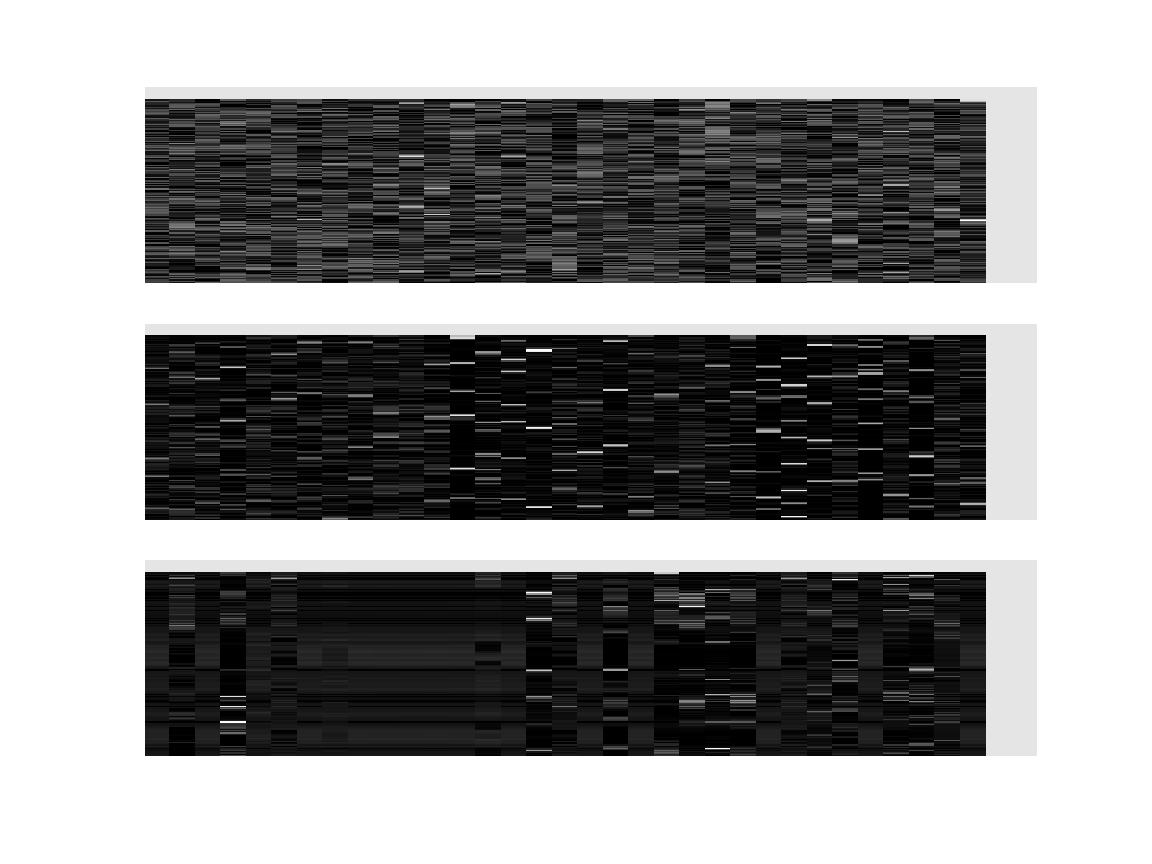
\includegraphics[scale=0.18]{./figures/basis}
		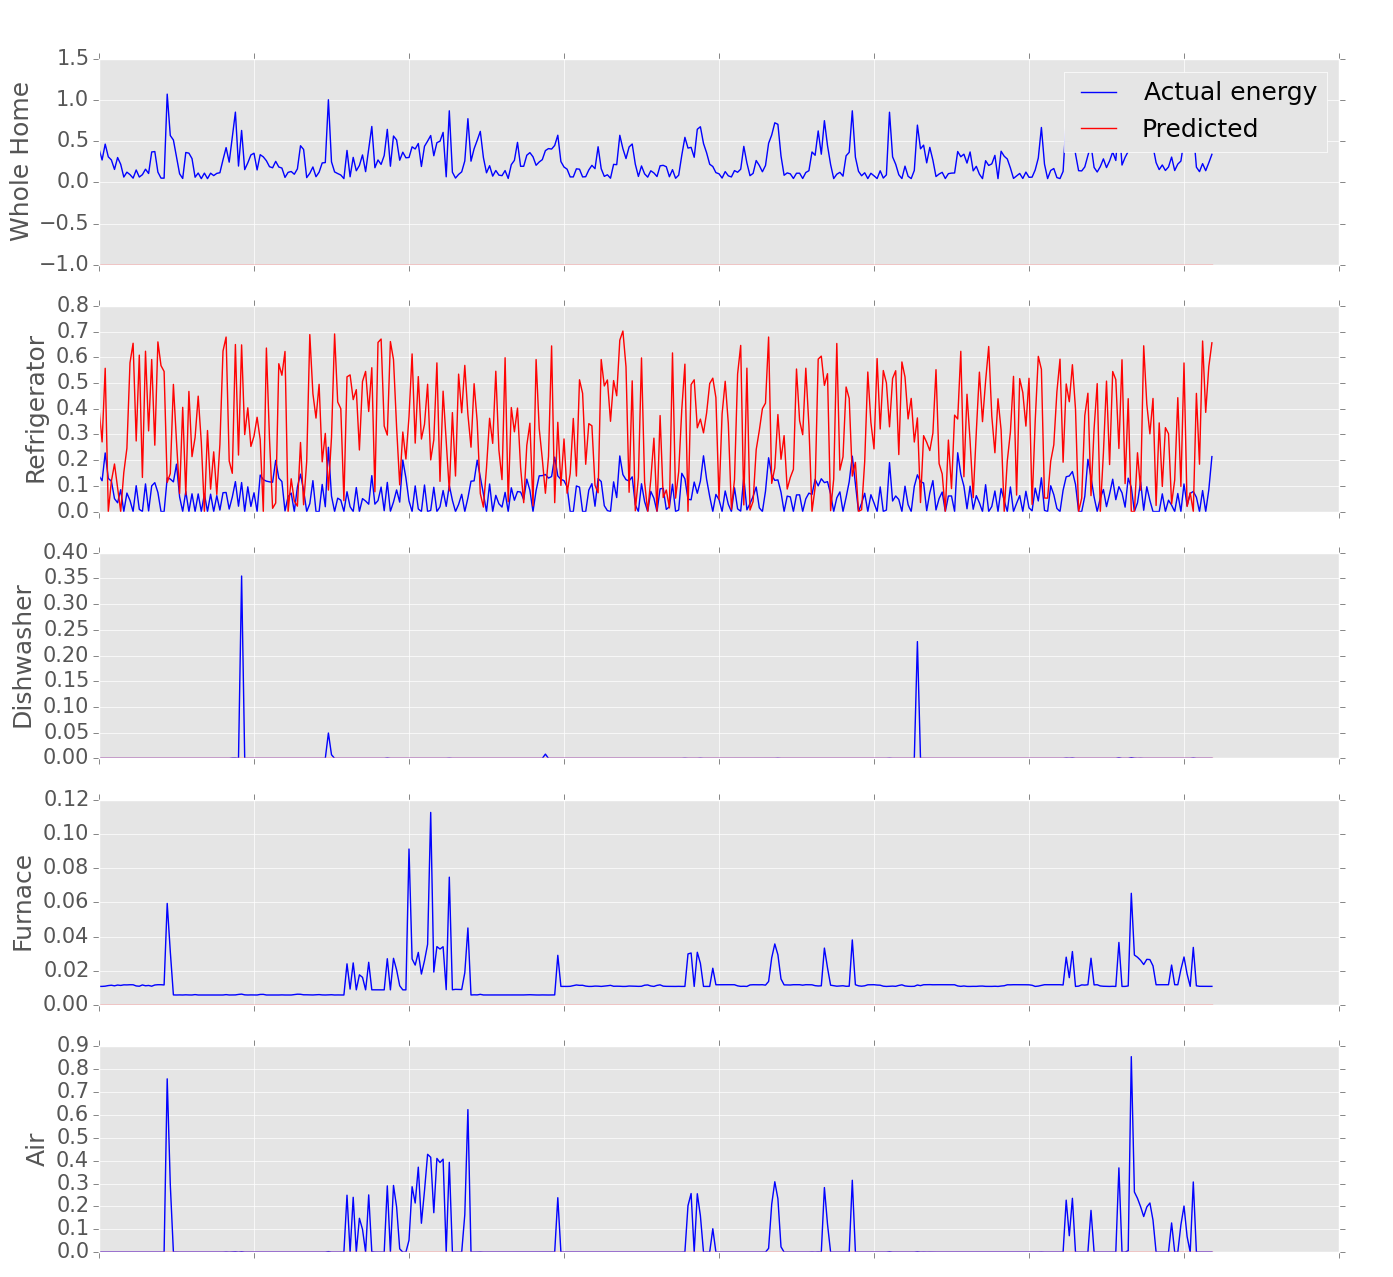
\includegraphics[scale=.18]{./figures/results/end_appliances_144_360}
	\end{minipage}
	\caption{Prediction of the weekday (top plots) and weekend (bottom plots) dataset.}
	\label{fig:days_end}
\end{figure}

The figure \ref{fig:days_end} shows that the predictions have not been successful when it comes to the datasets of weekdays and weekends. It has predicted that only a few appliances use energy. The only successful prediction is the dataset of weekdays for predicting two weeks of consumption. One thing to note is that the prediction of the air-condition for this dataset is the best prediction of all of the tests. It follows the consumption fairly well, and could be a consequence of the usage of air-condition being more homogenous during weekdays than during a whole week. The weekend dataset has the worst prediction of all the datasets, it also preferred to choose one appliance when predicting for two weeks as the week dataset. The prediction failure for the split datasets could be a result of a diminishing of training data, as the splitting of the dataset also made the training set smaller which could be the cause of the bad predictions.

\subsubsection{Basis functions}
\label{sec:a_b}
In addition to the disaggregation results themselves, sparse coding representations of the different device types are interesting in their own right, as they give a good intuition about how the different devices are typically used. The figure \ref{fig:basis_functions} shows a graphical representation of the learned basis functions. In each plot, the gray scale image on the right shows an intensity map of all bases functions learned for that device category, where each column in the image corresponds to a learned basis. 

\begin{figure}[H]
	\begin{center}

	\begin{minipage}{.5\textwidth}
		\centering
		%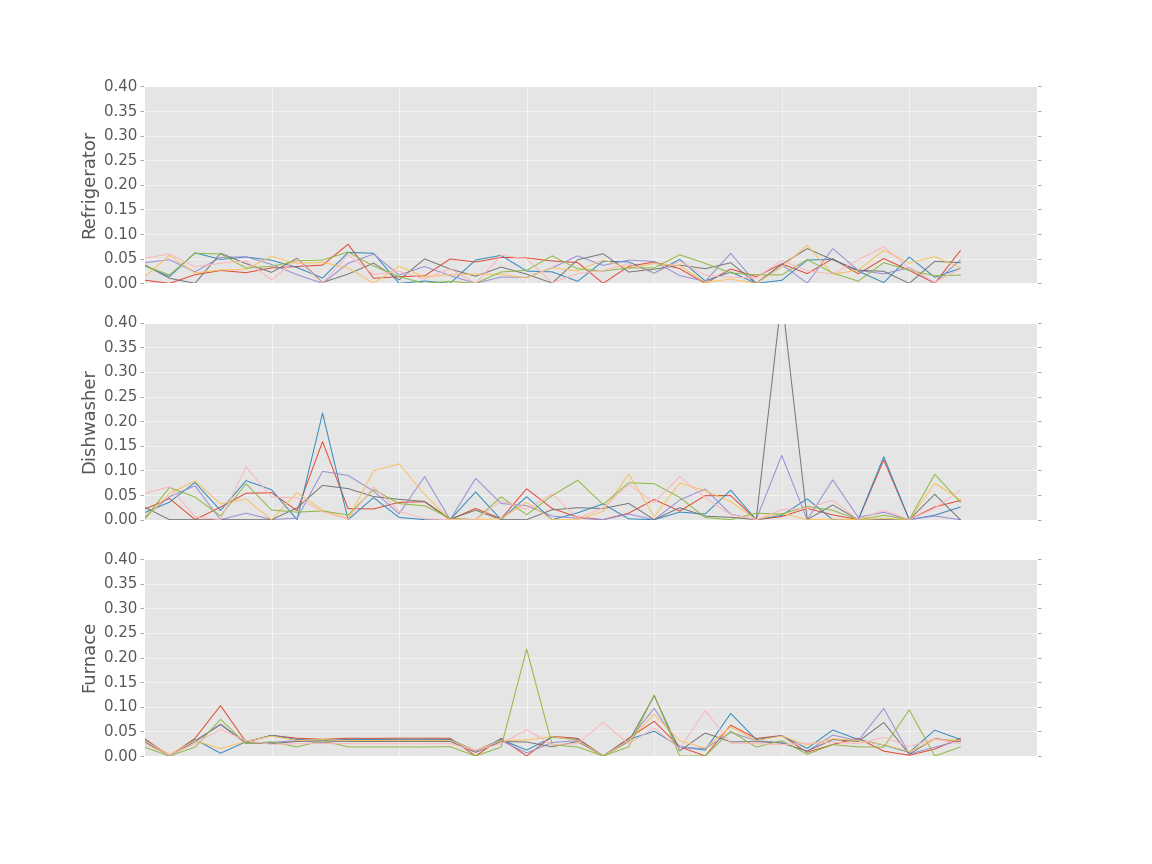
\includegraphics[scale=0.18]{./figures/app_basis}
		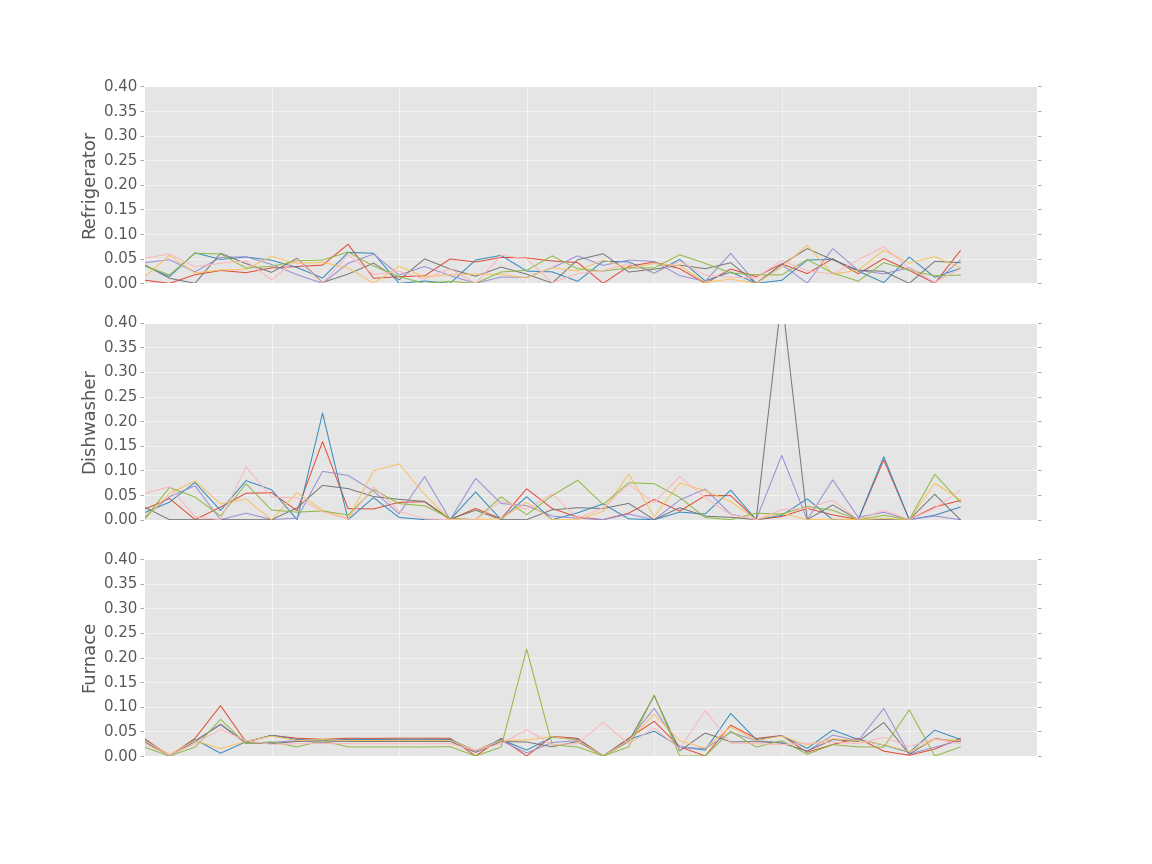
\includegraphics[width=\textwidth,height=12cm]{./figures/app_basis}
		\label{fig:test1}
	\end{minipage}%
	\begin{minipage}{.5\textwidth}
		\centering
		%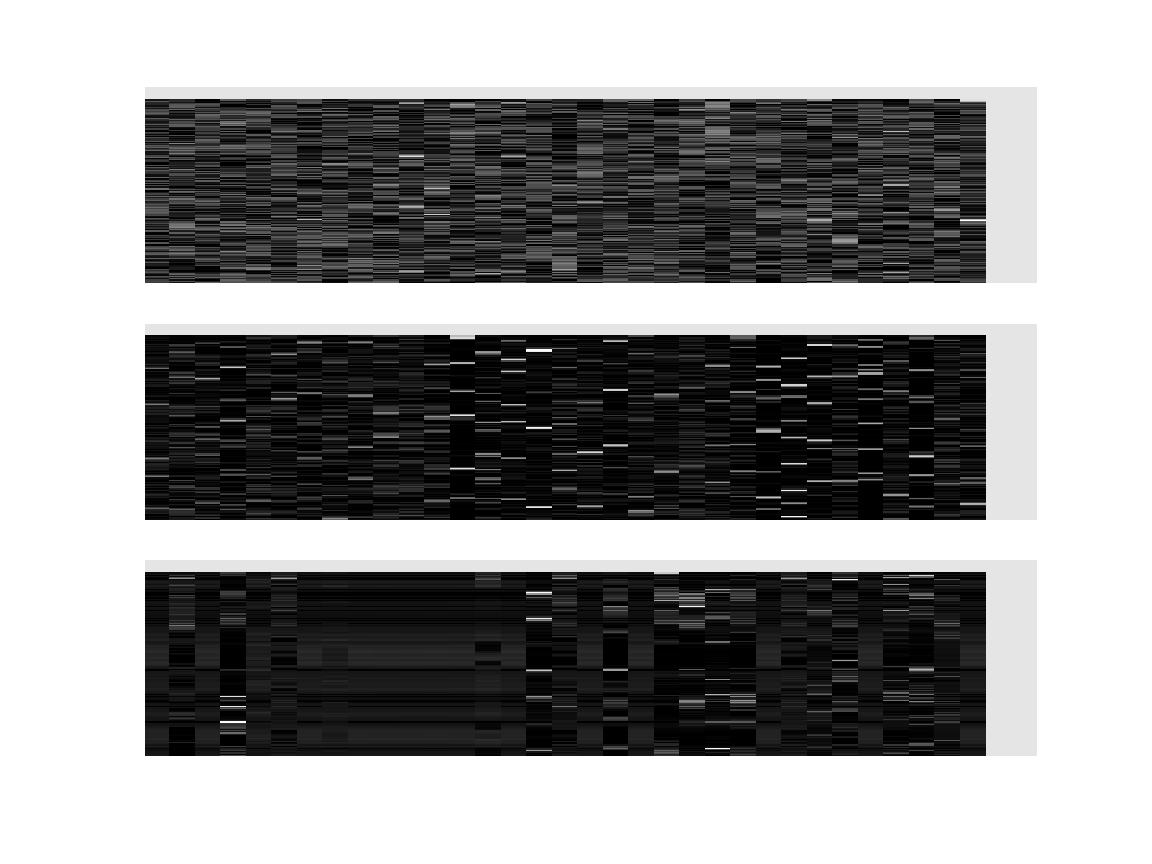
\includegraphics[scale=0.18]{./figures/basis}
		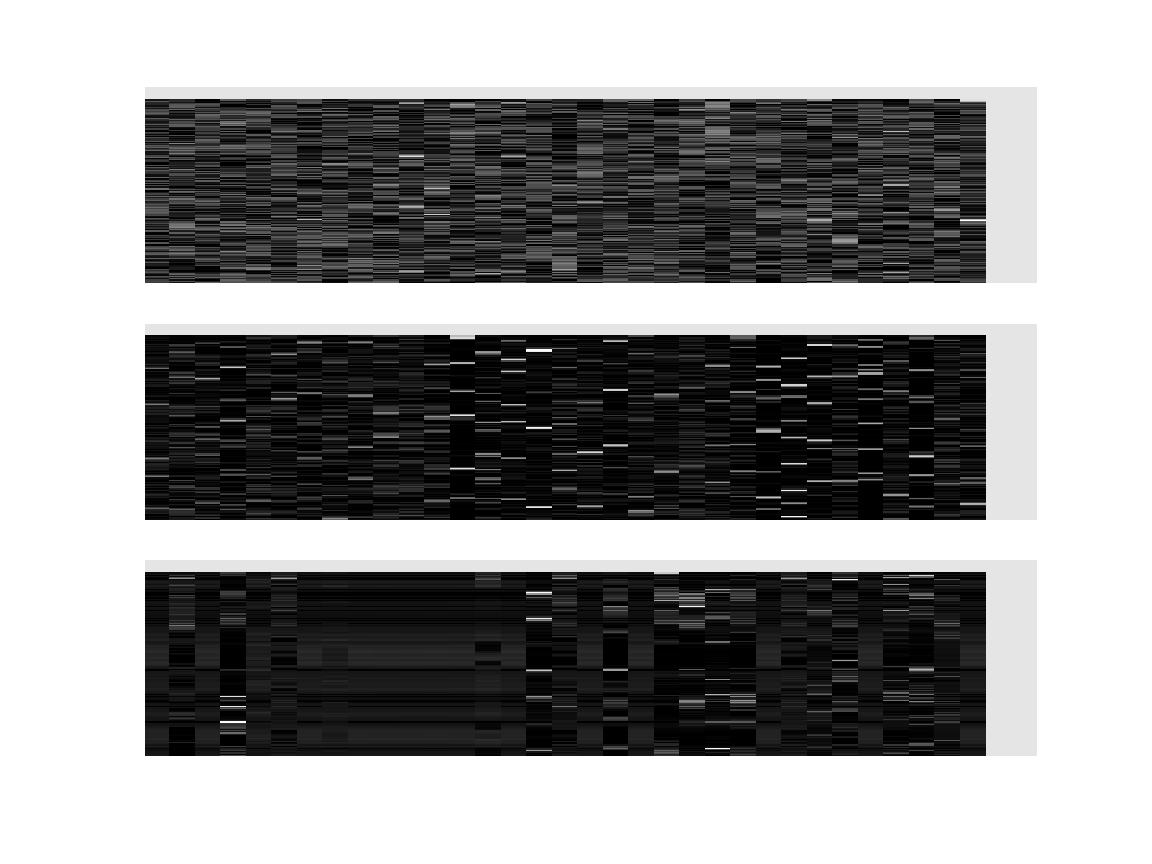
\includegraphics[width=\textwidth,height=12cm]{./figures/basis}
		\label{fig:test2}
	\end{minipage}
	\caption{Example basis functions learned from one device. The plots to the left shows seven example bases, while the image to the right shows all learned basis functions.}
	\label{fig:basis_functions}
	\end{center}
\end{figure}

The plots to the left shows seven examples of basis function for each of the devices. By interpreting the basis functions one can see that refrigerator has a more continuous function applied to it, in contrast to the dishwasher, which has a peak attached to it. This indicates that the functions have captured behaviors, such as "on" and "off" of the refrigerator compared to both the furnace and refrigerator, which in turn we assume do not have "on" and "off" behavior. Kotler et. al. \cite{DDSC} also got basis functions more peaked for refrigerator, which indicate that the basis functions are reasonably representative. They have more heavily peaked functions, which could be from their intense training. It can be said about the furnace, which has some basis that have a peak, which could correspond to a use of the furnace for a temporarily heating of the household. The magnitude of the refrigerator is lower than that of a dishwasher, which says that we have also captured the intensity of power consumption.

The right plots show that the refrigerator is "on" most of the time but with low power as we can see that the plot has mostly grey and some black in it. We can see that the dishwasher has peaked behavior in that some of the basis are almost pure white and some are black. We find interesting behaviors in the representations of the furnace as some of the basis fucntions really do look the same indicating that some furnaces behave similar and in similar magnitude.

\subsection{Quantitative evaluation of the Disaggregation}
\label{sec:quant}

There are a number of components to the final algorithm, and in this section we present quantitative results that evaluate the performance of each of these different algorithms. The most natural metric for evaluating disaggregation performance is the disaggregation error in equation \ref{eq:diserr}, i.e. the overlap of the pie charts of true and predicted percentage energy consumption shown in the figures \ref{fig:normal_168}, \ref{fig:normal_360}. While many of the arguments can be put into the temporal difference, we show that the algorithm has not been able to find a local optimum either by not having a parameter search or training data have not been sufficient. Moreover, the average disaggregation error presented in equation \ref{eq:acc} is not a particularly intuitive metric, and so we also evaluate a total time period accuracy of the prediction system, defined formally as

\begin{equation}
\label{eq:acc}
\text{Accuracy} \vcentcolon=  \frac{\sum_{i,q} \min \left\{ \sum_p ( \mathbf{X}_i)_{pq}, \sum_p ( \mathbf{B}_i,\hat{\mathbf{A}}_i)_{pq} \right\}}{\sum_{p,q} \bar{\mathbf{X}_i}_{p,q}}
\end{equation}

Despite the complex definition, this quantity simply captures the average amount of energy predicted correctly over the time period (i.e., the overlap between the actual and predicted energy).

\begin{figure}[H]
	\centering
	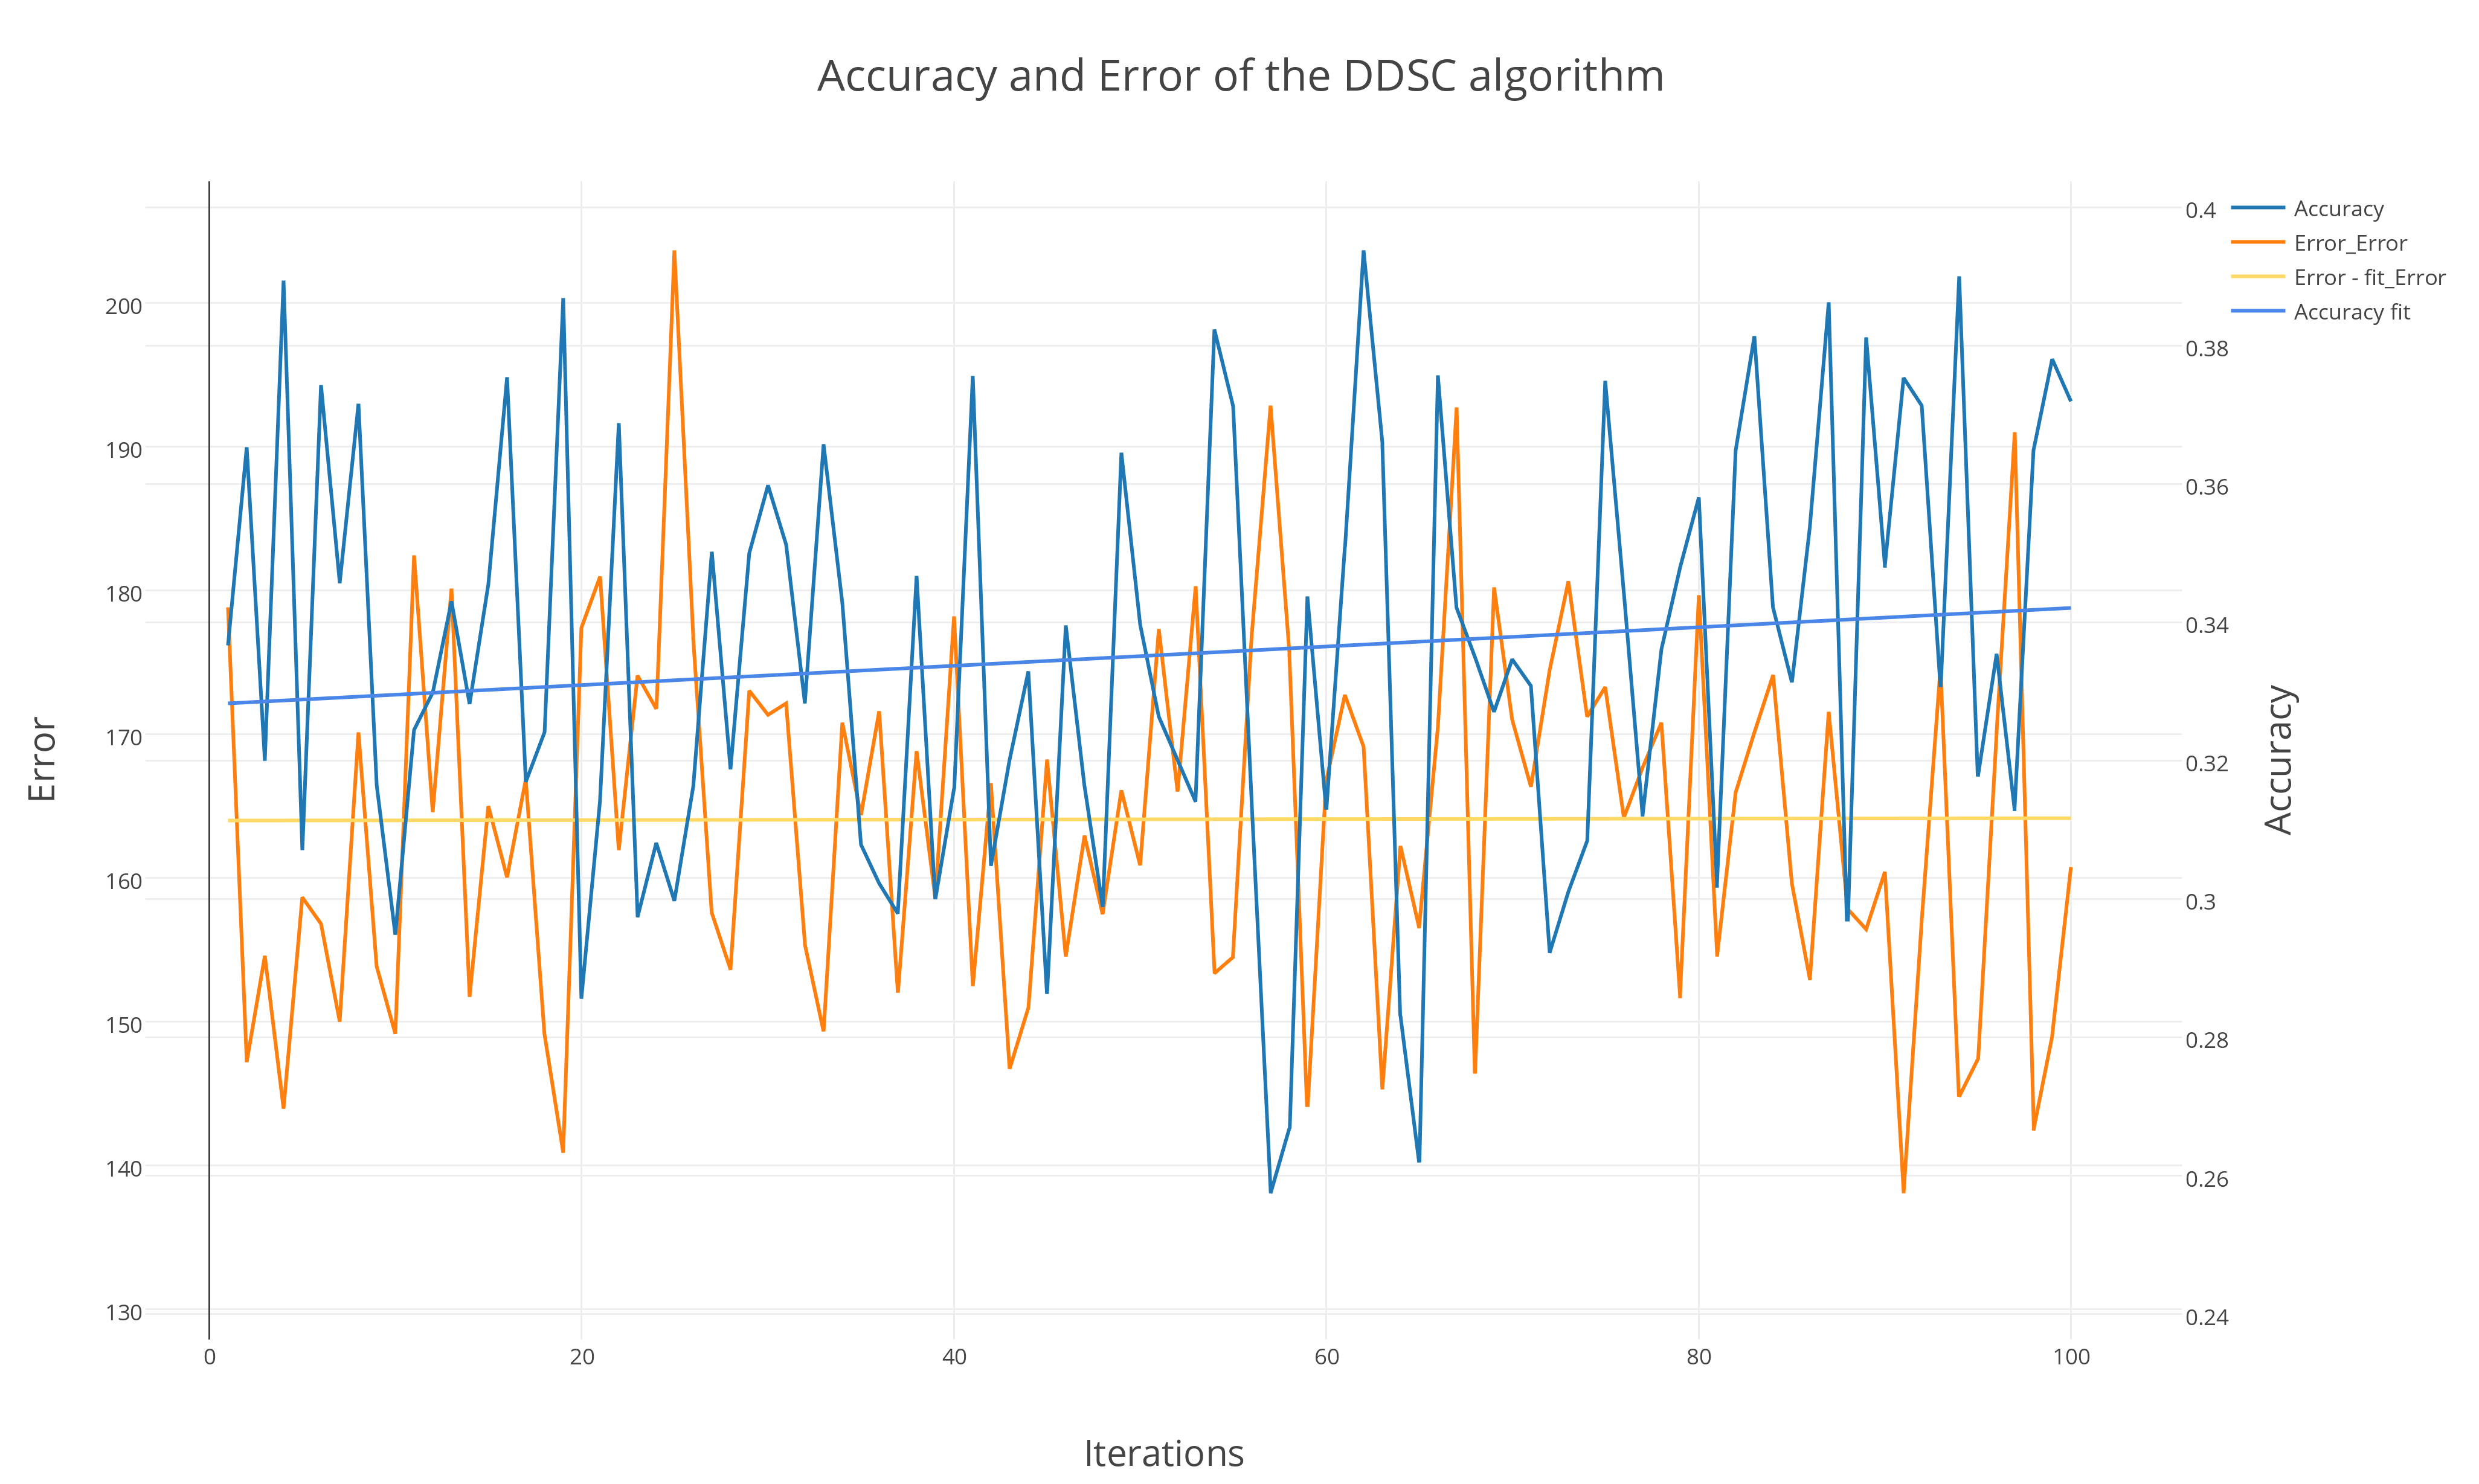
\includegraphics[scale=0.45]{./figures/acc_err_ddsc}
	\caption{Evolution of the training accuracy and error for the DDSC updates. The figure shows the best prediction of all the runs of the algorithm.}
	\label{fig:acc_err_ddsc}
\end{figure}

Figure \ref{fig:acc_err_ddsc} shows the disaggregation performance for the DDSC algorithm \ref{alg:ddsc}. It presents the disaggregation error from equation \ref{eq:diserr} on the left y-axis and the accuracy given in equation \ref{eq:acc} on the right y-axis. Furthermore a linear regression has been done for both the error and accuracy. We note that the accuracy is around 35\% following the fitted line when the 100:th iteration has been done. From the figure we see that for each iteration, the algorithm has difficulty finding an optimal path towards a minimization as seen by the volatile behavior of both the error and accuracy. However, fitting a curve to the values, we see that the accuracy has a positive slope although with regards to a high variance for curve fitting, the plot shows that we cannot fully rely on the implementation due to its behavior. Investigating this further, we took a look at the activation and basis norms of the algorithm. This yielded the following figure.

\begin{figure}[H]

	\centering
	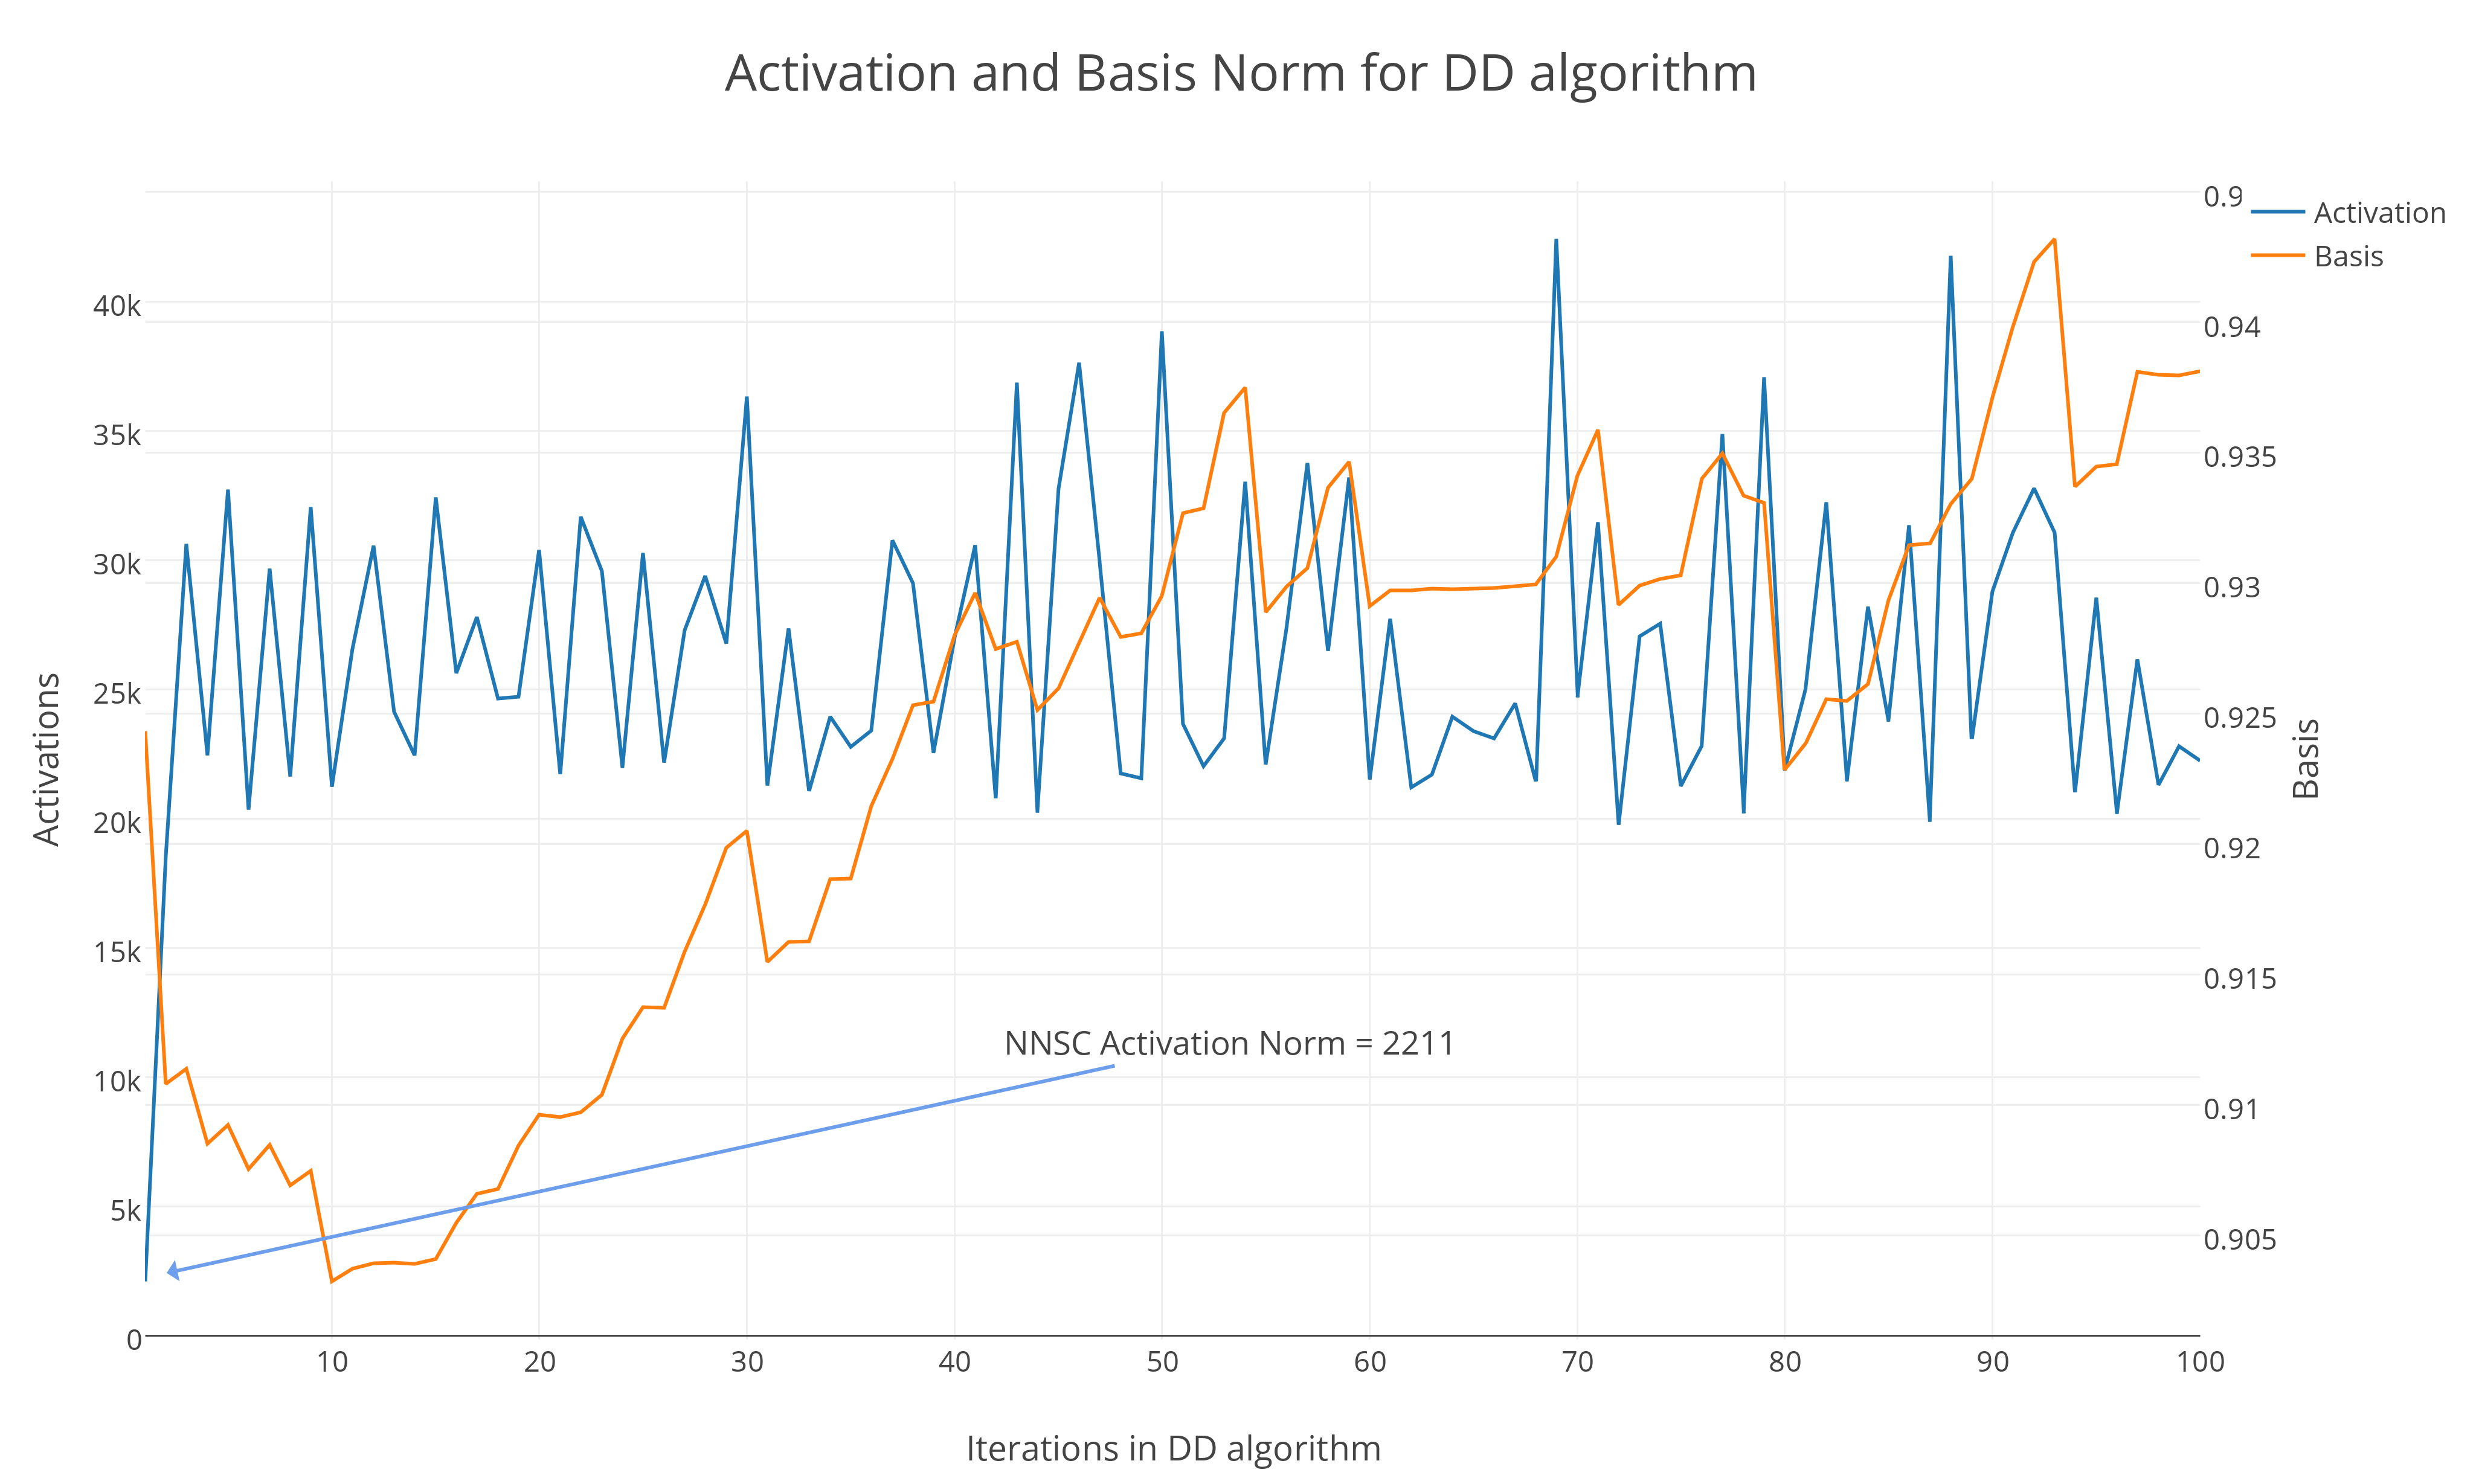
\includegraphics[scale=0.45]{./figures/a_b_norm}
	\caption{Evolution of the Activation and Basis norms for the DDSC updates. The norm of the Activations are seen on the left y-axis and the left y-axis is the Basis norm.}
	\label{fig:a_b_ddsc}
\end{figure}

The NNSC algorithm trains its activations separately for all of the appliances and yielded a norm of 2211 cumulatively for all of the appliances. We can see from the plot that when we start the DDSC algorithm the activation norms go from 2211 to around 25 000, which is probably due to the activations trying to adapt to the whole home energy consumption, which is vastly larger than each appliance. Interesting to note is that the basis norm slightly increases with each iteration, while the activations oscillate around 25 000. The activations trained are not used for the predicting the values for a new dataset, from this iteration we only take out the basis matrix which seems to have adapted itself by changing from a norm of 0.925 to 0.94.
